\documentclass[twoside]{book}

% Packages required by doxygen
\usepackage{fixltx2e}
\usepackage{calc}
\usepackage{doxygen}
\usepackage{graphicx}
\usepackage[utf8]{inputenc}
\usepackage{makeidx}
\usepackage{multicol}
\usepackage{multirow}
\PassOptionsToPackage{warn}{textcomp}
\usepackage{textcomp}
\usepackage[nointegrals]{wasysym}
\usepackage[table]{xcolor}

% Font selection
\usepackage[T1]{fontenc}
\usepackage{mathptmx}
\usepackage[scaled=.90]{helvet}
\usepackage{courier}
\usepackage{amssymb}
\usepackage{sectsty}
\renewcommand{\familydefault}{\sfdefault}
\allsectionsfont{%
  \fontseries{bc}\selectfont%
  \color{darkgray}%
}
\renewcommand{\DoxyLabelFont}{%
  \fontseries{bc}\selectfont%
  \color{darkgray}%
}
\newcommand{\+}{\discretionary{\mbox{\scriptsize$\hookleftarrow$}}{}{}}

% Page & text layout
\usepackage{geometry}
\geometry{%
  a4paper,%
  top=2.5cm,%
  bottom=2.5cm,%
  left=2.5cm,%
  right=2.5cm%
}
\tolerance=750
\hfuzz=15pt
\hbadness=750
\setlength{\emergencystretch}{15pt}
\setlength{\parindent}{0cm}
\setlength{\parskip}{0.2cm}
\makeatletter
\renewcommand{\paragraph}{%
  \@startsection{paragraph}{4}{0ex}{-1.0ex}{1.0ex}{%
    \normalfont\normalsize\bfseries\SS@parafont%
  }%
}
\renewcommand{\subparagraph}{%
  \@startsection{subparagraph}{5}{0ex}{-1.0ex}{1.0ex}{%
    \normalfont\normalsize\bfseries\SS@subparafont%
  }%
}
\makeatother

% Headers & footers
\usepackage{fancyhdr}
\pagestyle{fancyplain}
\fancyhead[LE]{\fancyplain{}{\bfseries\thepage}}
\fancyhead[CE]{\fancyplain{}{}}
\fancyhead[RE]{\fancyplain{}{\bfseries\leftmark}}
\fancyhead[LO]{\fancyplain{}{\bfseries\rightmark}}
\fancyhead[CO]{\fancyplain{}{}}
\fancyhead[RO]{\fancyplain{}{\bfseries\thepage}}
\fancyfoot[LE]{\fancyplain{}{}}
\fancyfoot[CE]{\fancyplain{}{}}
\fancyfoot[RE]{\fancyplain{}{\bfseries\scriptsize Generated on Mon Mar 26 2018 16\+:12\+:23 for Project Codename Olympia by Doxygen }}
\fancyfoot[LO]{\fancyplain{}{\bfseries\scriptsize Generated on Mon Mar 26 2018 16\+:12\+:23 for Project Codename Olympia by Doxygen }}
\fancyfoot[CO]{\fancyplain{}{}}
\fancyfoot[RO]{\fancyplain{}{}}
\renewcommand{\footrulewidth}{0.4pt}
\renewcommand{\chaptermark}[1]{%
  \markboth{#1}{}%
}
\renewcommand{\sectionmark}[1]{%
  \markright{\thesection\ #1}%
}

% Indices & bibliography
\usepackage{natbib}
\usepackage[titles]{tocloft}
\setcounter{tocdepth}{3}
\setcounter{secnumdepth}{5}
\makeindex

% Hyperlinks (required, but should be loaded last)
\usepackage{ifpdf}
\ifpdf
  \usepackage[pdftex,pagebackref=true]{hyperref}
\else
  \usepackage[ps2pdf,pagebackref=true]{hyperref}
\fi
\hypersetup{%
  colorlinks=true,%
  linkcolor=blue,%
  citecolor=blue,%
  unicode%
}

% Custom commands
\newcommand{\clearemptydoublepage}{%
  \newpage{\pagestyle{empty}\cleardoublepage}%
}


%===== C O N T E N T S =====

\begin{document}

% Titlepage & ToC
\hypersetup{pageanchor=false,
             bookmarks=true,
             bookmarksnumbered=true,
             pdfencoding=unicode
            }
\pagenumbering{roman}
\begin{titlepage}
\vspace*{7cm}
\begin{center}%
{\Large Project Codename Olympia }\\
\vspace*{1cm}
{\large Generated by Doxygen 1.8.8}\\
\vspace*{0.5cm}
{\small Mon Mar 26 2018 16:12:23}\\
\end{center}
\end{titlepage}
\clearemptydoublepage
\tableofcontents
\clearemptydoublepage
\pagenumbering{arabic}
\hypersetup{pageanchor=true}

%--- Begin generated contents ---
\chapter{Namespace Index}
\section{Namespace List}
Here is a list of all documented namespaces with brief descriptions\+:\begin{DoxyCompactList}
\item\contentsline{section}{\hyperlink{namespaceProject__Codename__Olympia__v1}{Project\+\_\+\+Codename\+\_\+\+Olympia\+\_\+v1} }{\pageref{namespaceProject__Codename__Olympia__v1}}{}
\item\contentsline{section}{\hyperlink{namespaceProject__Codename__Olympia__v1_1_1__0}{Project\+\_\+\+Codename\+\_\+\+Olympia\+\_\+v1.\+\_\+0} }{\pageref{namespaceProject__Codename__Olympia__v1_1_1__0}}{}
\end{DoxyCompactList}

\chapter{Class Index}
\section{Class List}
Here are the classes, structs, unions and interfaces with brief descriptions\+:\begin{DoxyCompactList}
\item\contentsline{section}{\hyperlink{classPCO_1_1Athlete}{P\+C\+O.\+Athlete} \\*\hyperlink{classPCO_1_1Athlete}{Athlete} class to input individual's personal information and events to partake in }{\pageref{classPCO_1_1Athlete}}{}
\item\contentsline{section}{\hyperlink{classPCO_1_1Database}{P\+C\+O.\+Database} \\*D\+E\+P\+R\+E\+C\+A\+T\+E\+D!!! \hyperlink{classPCO_1_1Database}{Database} S\+U\+B\+S\+Y\+S\+T\+E\+M houses all the information of the Winter Olympics }{\pageref{classPCO_1_1Database}}{}
\item\contentsline{section}{\hyperlink{classPCO_1_1Event}{P\+C\+O.\+Event} \\*\hyperlink{classPCO_1_1Event}{Event} class is the superclass of all the 2 event types and 6 specific events }{\pageref{classPCO_1_1Event}}{}
\item\contentsline{section}{\hyperlink{interfacePCO_1_1Event_1_1eventInheritance}{P\+C\+O.\+Event.\+event\+Inheritance} }{\pageref{interfacePCO_1_1Event_1_1eventInheritance}}{}
\item\contentsline{section}{\hyperlink{classPCO_1_1FigureSkating}{P\+C\+O.\+Figure\+Skating} \\*\hyperlink{classPCO_1_1FigureSkating}{Figure\+Skating} class is the superclass of the 3 \hyperlink{classPCO_1_1FigureSkating}{Figure\+Skating} events }{\pageref{classPCO_1_1FigureSkating}}{}
\item\contentsline{section}{\hyperlink{interfacePCO_1_1FigureSkating_1_1fsInheritance}{P\+C\+O.\+Figure\+Skating.\+fs\+Inheritance} }{\pageref{interfacePCO_1_1FigureSkating_1_1fsInheritance}}{}
\item\contentsline{section}{\hyperlink{classPCO_1_1IceDance}{P\+C\+O.\+Ice\+Dance} \\*\hyperlink{classPCO_1_1IceDance}{Ice\+Dance} class is one of the 3 \hyperlink{classPCO_1_1FigureSkating}{Figure\+Skating} events }{\pageref{classPCO_1_1IceDance}}{}
\item\contentsline{section}{\hyperlink{classPCO_1_1Judge}{P\+C\+O.\+Judge} \\*\hyperlink{classPCO_1_1Judge}{Judge} class houses and disperses all the qualified judges }{\pageref{classPCO_1_1Judge}}{}
\item\contentsline{section}{\hyperlink{classPCO_1_1MainClass}{P\+C\+O.\+Main\+Class} }{\pageref{classPCO_1_1MainClass}}{}
\item\contentsline{section}{\hyperlink{classPCO_1_1PairSkating}{P\+C\+O.\+Pair\+Skating} \\*\hyperlink{classPCO_1_1PairSkating}{Pair\+Skating} class is one of the 3 \hyperlink{classPCO_1_1FigureSkating}{Figure\+Skating} events }{\pageref{classPCO_1_1PairSkating}}{}
\item\contentsline{section}{\hyperlink{classPCO_1_1Registration}{P\+C\+O.\+Registration} \\*\hyperlink{classPCO_1_1Registration}{Registration} class registers Teams and Athletes }{\pageref{classPCO_1_1Registration}}{}
\item\contentsline{section}{\hyperlink{classPCO_1_1Rink}{P\+C\+O.\+Rink} \\*\hyperlink{classPCO_1_1Rink}{Rink} class is the physical area in which events are held }{\pageref{classPCO_1_1Rink}}{}
\item\contentsline{section}{\hyperlink{classPCO_1_1Schedule}{P\+C\+O.\+Schedule} \\*\hyperlink{classPCO_1_1Schedule}{Schedule} class is the organization of athletes and events }{\pageref{classPCO_1_1Schedule}}{}
\item\contentsline{section}{\hyperlink{classPCO_1_1Scoring}{P\+C\+O.\+Scoring} \\*\hyperlink{classPCO_1_1Scoring}{Scoring} class manages the official scores/times recorded by the judges }{\pageref{classPCO_1_1Scoring}}{}
\item\contentsline{section}{\hyperlink{classPCO_1_1SingleSkating}{P\+C\+O.\+Single\+Skating} \\*\hyperlink{classPCO_1_1SingleSkating}{Single\+Skating} class is one of the 3 \hyperlink{classPCO_1_1FigureSkating}{Figure\+Skating} events }{\pageref{classPCO_1_1SingleSkating}}{}
\item\contentsline{section}{\hyperlink{classPCO_1_1SpeedSkating}{P\+C\+O.\+Speed\+Skating} \\*\hyperlink{classPCO_1_1SpeedSkating}{Speed\+Skating} class is the superclass of the 3 \hyperlink{classPCO_1_1SpeedSkating}{Speed\+Skating} events }{\pageref{classPCO_1_1SpeedSkating}}{}
\item\contentsline{section}{\hyperlink{classPCO_1_1SS1000m}{P\+C\+O.\+S\+S1000m} \\*\hyperlink{classPCO_1_1SS1000m}{S\+S1000m} is one of the 3 \hyperlink{classPCO_1_1SpeedSkating}{Speed\+Skating} events }{\pageref{classPCO_1_1SS1000m}}{}
\item\contentsline{section}{\hyperlink{classPCO_1_1SS1500m}{P\+C\+O.\+S\+S1500m} \\*\hyperlink{classPCO_1_1SS1500m}{S\+S1500m} is one of the 3 \hyperlink{classPCO_1_1SpeedSkating}{Speed\+Skating} events }{\pageref{classPCO_1_1SS1500m}}{}
\item\contentsline{section}{\hyperlink{classPCO_1_1SS500m}{P\+C\+O.\+S\+S500m} \\*\hyperlink{classPCO_1_1SS500m}{S\+S500m} is one of the 3 \hyperlink{classPCO_1_1SpeedSkating}{Speed\+Skating} events }{\pageref{classPCO_1_1SS500m}}{}
\item\contentsline{section}{\hyperlink{interfacePCO_1_1SpeedSkating_1_1ssInheritance}{P\+C\+O.\+Speed\+Skating.\+ss\+Inheritance} }{\pageref{interfacePCO_1_1SpeedSkating_1_1ssInheritance}}{}
\item\contentsline{section}{\hyperlink{classPCO_1_1Team}{P\+C\+O.\+Team} \\*\hyperlink{classPCO_1_1Team}{Team} class to house the team name }{\pageref{classPCO_1_1Team}}{}
\end{DoxyCompactList}

\chapter{File Index}
\section{File List}
Here is a list of all files with brief descriptions\+:\begin{DoxyCompactList}
\item\contentsline{section}{\hyperlink{Class1_8cs}{Class1.\+cs} }{\pageref{Class1_8cs}}{}
\item\contentsline{section}{\hyperlink{Display_8cs}{Display.\+cs} }{\pageref{Display_8cs}}{}
\item\contentsline{section}{\hyperlink{Display_8Designer_8cs}{Display.\+Designer.\+cs} }{\pageref{Display_8Designer_8cs}}{}
\item\contentsline{section}{\hyperlink{Event_8cs}{Event.\+cs} }{\pageref{Event_8cs}}{}
\item\contentsline{section}{\hyperlink{Event_8Designer_8cs}{Event.\+Designer.\+cs} }{\pageref{Event_8Designer_8cs}}{}
\item\contentsline{section}{\hyperlink{Form1_8cs}{Form1.\+cs} }{\pageref{Form1_8cs}}{}
\item\contentsline{section}{\hyperlink{Form1_8Designer_8cs}{Form1.\+Designer.\+cs} }{\pageref{Form1_8Designer_8cs}}{}
\item\contentsline{section}{\hyperlink{Judge_8cs}{Judge.\+cs} }{\pageref{Judge_8cs}}{}
\item\contentsline{section}{\hyperlink{Judge_8Designer_8cs}{Judge.\+Designer.\+cs} }{\pageref{Judge_8Designer_8cs}}{}
\item\contentsline{section}{\hyperlink{Program_8cs}{Program.\+cs} }{\pageref{Program_8cs}}{}
\item\contentsline{section}{\hyperlink{Registration_8cs}{Registration.\+cs} }{\pageref{Registration_8cs}}{}
\item\contentsline{section}{\hyperlink{Registration_8Designer_8cs}{Registration.\+Designer.\+cs} }{\pageref{Registration_8Designer_8cs}}{}
\item\contentsline{section}{\hyperlink{Team_8cs}{Team.\+cs} }{\pageref{Team_8cs}}{}
\item\contentsline{section}{\hyperlink{Team_8Designer_8cs}{Team.\+Designer.\+cs} }{\pageref{Team_8Designer_8cs}}{}
\end{DoxyCompactList}

\chapter{Namespace Documentation}
\hypertarget{namespacePCO}{\section{Package P\+C\+O}
\label{namespacePCO}\index{P\+C\+O@{P\+C\+O}}
}
\subsection*{Classes}
\begin{DoxyCompactItemize}
\item 
class \hyperlink{classPCO_1_1Athlete}{Athlete}
\begin{DoxyCompactList}\small\item\em \hyperlink{classPCO_1_1Athlete}{Athlete} class to input individual's personal information and events to partake in. \end{DoxyCompactList}\item 
class \hyperlink{classPCO_1_1Database}{Database}
\begin{DoxyCompactList}\small\item\em D\+E\+P\+R\+E\+C\+A\+T\+E\+D!!! \hyperlink{classPCO_1_1Database}{Database} S\+U\+B\+S\+Y\+S\+T\+E\+M houses all the information of the Winter Olympics. \end{DoxyCompactList}\item 
class \hyperlink{classPCO_1_1Event}{Event}
\begin{DoxyCompactList}\small\item\em \hyperlink{classPCO_1_1Event}{Event} class is the superclass of all the 2 event types and 6 specific events. \end{DoxyCompactList}\item 
class \hyperlink{classPCO_1_1FigureSkating}{Figure\+Skating}
\begin{DoxyCompactList}\small\item\em \hyperlink{classPCO_1_1FigureSkating}{Figure\+Skating} class is the superclass of the 3 \hyperlink{classPCO_1_1FigureSkating}{Figure\+Skating} events. \end{DoxyCompactList}\item 
class \hyperlink{classPCO_1_1IceDance}{Ice\+Dance}
\begin{DoxyCompactList}\small\item\em \hyperlink{classPCO_1_1IceDance}{Ice\+Dance} class is one of the 3 \hyperlink{classPCO_1_1FigureSkating}{Figure\+Skating} events. \end{DoxyCompactList}\item 
class \hyperlink{classPCO_1_1Judge}{Judge}
\begin{DoxyCompactList}\small\item\em \hyperlink{classPCO_1_1Judge}{Judge} class houses and disperses all the qualified judges. \end{DoxyCompactList}\item 
class \hyperlink{classPCO_1_1MainClass}{Main\+Class}
\item 
class \hyperlink{classPCO_1_1PairSkating}{Pair\+Skating}
\begin{DoxyCompactList}\small\item\em \hyperlink{classPCO_1_1PairSkating}{Pair\+Skating} class is one of the 3 \hyperlink{classPCO_1_1FigureSkating}{Figure\+Skating} events. \end{DoxyCompactList}\item 
class \hyperlink{classPCO_1_1Registration}{Registration}
\begin{DoxyCompactList}\small\item\em \hyperlink{classPCO_1_1Registration}{Registration} class registers Teams and Athletes. \end{DoxyCompactList}\item 
class \hyperlink{classPCO_1_1Rink}{Rink}
\begin{DoxyCompactList}\small\item\em \hyperlink{classPCO_1_1Rink}{Rink} class is the physical area in which events are held. \end{DoxyCompactList}\item 
class \hyperlink{classPCO_1_1Schedule}{Schedule}
\begin{DoxyCompactList}\small\item\em \hyperlink{classPCO_1_1Schedule}{Schedule} class is the organization of athletes and events. \end{DoxyCompactList}\item 
class \hyperlink{classPCO_1_1Scoring}{Scoring}
\begin{DoxyCompactList}\small\item\em \hyperlink{classPCO_1_1Scoring}{Scoring} class manages the official scores/times recorded by the judges. \end{DoxyCompactList}\item 
class \hyperlink{classPCO_1_1SingleSkating}{Single\+Skating}
\begin{DoxyCompactList}\small\item\em \hyperlink{classPCO_1_1SingleSkating}{Single\+Skating} class is one of the 3 \hyperlink{classPCO_1_1FigureSkating}{Figure\+Skating} events. \end{DoxyCompactList}\item 
class \hyperlink{classPCO_1_1SpeedSkating}{Speed\+Skating}
\begin{DoxyCompactList}\small\item\em \hyperlink{classPCO_1_1SpeedSkating}{Speed\+Skating} class is the superclass of the 3 \hyperlink{classPCO_1_1SpeedSkating}{Speed\+Skating} events. \end{DoxyCompactList}\item 
class \hyperlink{classPCO_1_1SS1000m}{S\+S1000m}
\begin{DoxyCompactList}\small\item\em \hyperlink{classPCO_1_1SS1000m}{S\+S1000m} is one of the 3 \hyperlink{classPCO_1_1SpeedSkating}{Speed\+Skating} events. \end{DoxyCompactList}\item 
class \hyperlink{classPCO_1_1SS1500m}{S\+S1500m}
\begin{DoxyCompactList}\small\item\em \hyperlink{classPCO_1_1SS1500m}{S\+S1500m} is one of the 3 \hyperlink{classPCO_1_1SpeedSkating}{Speed\+Skating} events. \end{DoxyCompactList}\item 
class \hyperlink{classPCO_1_1SS500m}{S\+S500m}
\begin{DoxyCompactList}\small\item\em \hyperlink{classPCO_1_1SS500m}{S\+S500m} is one of the 3 \hyperlink{classPCO_1_1SpeedSkating}{Speed\+Skating} events. \end{DoxyCompactList}\item 
class \hyperlink{classPCO_1_1Team}{Team}
\begin{DoxyCompactList}\small\item\em \hyperlink{classPCO_1_1Team}{Team} class to house the team name. \end{DoxyCompactList}\end{DoxyCompactItemize}

\chapter{Class Documentation}
\hypertarget{classPCO_1_1Athlete}{\section{P\+C\+O.\+Athlete Class Reference}
\label{classPCO_1_1Athlete}\index{P\+C\+O.\+Athlete@{P\+C\+O.\+Athlete}}
}


\hyperlink{classPCO_1_1Athlete}{Athlete} class to input individual's personal information and events to partake in.  


\subsection*{Public Member Functions}
\begin{DoxyCompactItemize}
\item 
\hyperlink{classPCO_1_1Athlete_a65af66e3b9da62287fbcd73cb1903280}{Athlete} ()
\end{DoxyCompactItemize}
\subsection*{Properties}
\begin{DoxyCompactItemize}
\item 
string \hyperlink{classPCO_1_1Athlete_a6167fdc1ef5b40ec091f3c81a8da3a8c}{first\+Name}\hspace{0.3cm}{\ttfamily  \mbox{[}get, set\mbox{]}}
\item 
string \hyperlink{classPCO_1_1Athlete_a8585d7d2291f32ef95be2934840b734a}{last\+Name}\hspace{0.3cm}{\ttfamily  \mbox{[}get, set\mbox{]}}
\item 
string \hyperlink{classPCO_1_1Athlete_af1d423796bbb1680beb437ced0def7b4}{gender}\hspace{0.3cm}{\ttfamily  \mbox{[}get, set\mbox{]}}
\item 
\hyperlink{classPCO_1_1Schedule}{Schedule} \hyperlink{classPCO_1_1Athlete_a64a37dcb54d6428079498964da17801d}{set\+Schedule}\hspace{0.3cm}{\ttfamily  \mbox{[}get, set\mbox{]}}
\item 
Tuple$<$ int, int, int $>$ \hyperlink{classPCO_1_1Athlete_a99ff064c8d40bcb39a7dac132a9146e4}{medals}\hspace{0.3cm}{\ttfamily  \mbox{[}get, set\mbox{]}}
\end{DoxyCompactItemize}


\subsection{Detailed Description}
\hyperlink{classPCO_1_1Athlete}{Athlete} class to input individual's personal information and events to partake in. 

D\+E\+F\+I\+N\+I\+T\+I\+O\+N\+: An individual who is a part of a team in the Winter Olympics.

C\+O\+N\+S\+T\+R\+A\+I\+N\+T\+S\+: Can only be registered if maximum allotted space on their respective team has not been reached. This also includes the gender portion.\begin{DoxyAuthor}{Author}
Landen Marchand 
\end{DoxyAuthor}


Definition at line 14 of file Athlete.\+cs.



\subsection{Constructor \& Destructor Documentation}
\hypertarget{classPCO_1_1Athlete_a65af66e3b9da62287fbcd73cb1903280}{\index{P\+C\+O\+::\+Athlete@{P\+C\+O\+::\+Athlete}!Athlete@{Athlete}}
\index{Athlete@{Athlete}!P\+C\+O\+::\+Athlete@{P\+C\+O\+::\+Athlete}}
\subsubsection[{Athlete}]{\setlength{\rightskip}{0pt plus 5cm}P\+C\+O.\+Athlete.\+Athlete (
\begin{DoxyParamCaption}
{}
\end{DoxyParamCaption}
)\hspace{0.3cm}{\ttfamily [inline]}}}\label{classPCO_1_1Athlete_a65af66e3b9da62287fbcd73cb1903280}
Default Constructor Provided Automatically 
\begin{DoxyParams}{Parameters}
{\em None} & \\
\hline
\end{DoxyParams}
\begin{DoxyReturn}{Returns}
Default Values 
\end{DoxyReturn}


Definition at line 20 of file Athlete.\+cs.



\subsection{Property Documentation}
\hypertarget{classPCO_1_1Athlete_a6167fdc1ef5b40ec091f3c81a8da3a8c}{\index{P\+C\+O\+::\+Athlete@{P\+C\+O\+::\+Athlete}!first\+Name@{first\+Name}}
\index{first\+Name@{first\+Name}!P\+C\+O\+::\+Athlete@{P\+C\+O\+::\+Athlete}}
\subsubsection[{first\+Name}]{\setlength{\rightskip}{0pt plus 5cm}string P\+C\+O.\+Athlete.\+first\+Name\hspace{0.3cm}{\ttfamily [get]}, {\ttfamily [set]}}}\label{classPCO_1_1Athlete_a6167fdc1ef5b40ec091f3c81a8da3a8c}
Sets and gets athlete's first name 
\begin{DoxyParams}{Parameters}
{\em string} & for first name \\
\hline
\end{DoxyParams}
\begin{DoxyReturn}{Returns}
string of first name 
\end{DoxyReturn}


Definition at line 28 of file Athlete.\+cs.

\hypertarget{classPCO_1_1Athlete_af1d423796bbb1680beb437ced0def7b4}{\index{P\+C\+O\+::\+Athlete@{P\+C\+O\+::\+Athlete}!gender@{gender}}
\index{gender@{gender}!P\+C\+O\+::\+Athlete@{P\+C\+O\+::\+Athlete}}
\subsubsection[{gender}]{\setlength{\rightskip}{0pt plus 5cm}string P\+C\+O.\+Athlete.\+gender\hspace{0.3cm}{\ttfamily [get]}, {\ttfamily [set]}}}\label{classPCO_1_1Athlete_af1d423796bbb1680beb437ced0def7b4}
Sets and gets athlete's gender 
\begin{DoxyParams}{Parameters}
{\em string} & for gender \\
\hline
\end{DoxyParams}
\begin{DoxyReturn}{Returns}
string of gender 
\end{DoxyReturn}


Definition at line 38 of file Athlete.\+cs.

\hypertarget{classPCO_1_1Athlete_a8585d7d2291f32ef95be2934840b734a}{\index{P\+C\+O\+::\+Athlete@{P\+C\+O\+::\+Athlete}!last\+Name@{last\+Name}}
\index{last\+Name@{last\+Name}!P\+C\+O\+::\+Athlete@{P\+C\+O\+::\+Athlete}}
\subsubsection[{last\+Name}]{\setlength{\rightskip}{0pt plus 5cm}string P\+C\+O.\+Athlete.\+last\+Name\hspace{0.3cm}{\ttfamily [get]}, {\ttfamily [set]}}}\label{classPCO_1_1Athlete_a8585d7d2291f32ef95be2934840b734a}
Sets and gets athlete's last name 
\begin{DoxyParams}{Parameters}
{\em string} & for last name \\
\hline
\end{DoxyParams}
\begin{DoxyReturn}{Returns}
string of last name 
\end{DoxyReturn}


Definition at line 33 of file Athlete.\+cs.

\hypertarget{classPCO_1_1Athlete_a99ff064c8d40bcb39a7dac132a9146e4}{\index{P\+C\+O\+::\+Athlete@{P\+C\+O\+::\+Athlete}!medals@{medals}}
\index{medals@{medals}!P\+C\+O\+::\+Athlete@{P\+C\+O\+::\+Athlete}}
\subsubsection[{medals}]{\setlength{\rightskip}{0pt plus 5cm}Tuple$<$int,int,int$>$ P\+C\+O.\+Athlete.\+medals\hspace{0.3cm}{\ttfamily [get]}, {\ttfamily [set]}}}\label{classPCO_1_1Athlete_a99ff064c8d40bcb39a7dac132a9146e4}
Sets and gets athlete's medal count for gold/silver/bronze 
\begin{DoxyParams}{Parameters}
{\em Tuple$<$int,int,int$>$} & \\
\hline
\end{DoxyParams}
\begin{DoxyReturn}{Returns}
Tuple$<$int,int,int$>$ Gold,Silver,Bronze ints 
\end{DoxyReturn}


Definition at line 48 of file Athlete.\+cs.

\hypertarget{classPCO_1_1Athlete_a64a37dcb54d6428079498964da17801d}{\index{P\+C\+O\+::\+Athlete@{P\+C\+O\+::\+Athlete}!set\+Schedule@{set\+Schedule}}
\index{set\+Schedule@{set\+Schedule}!P\+C\+O\+::\+Athlete@{P\+C\+O\+::\+Athlete}}
\subsubsection[{set\+Schedule}]{\setlength{\rightskip}{0pt plus 5cm}{\bf Schedule} P\+C\+O.\+Athlete.\+set\+Schedule\hspace{0.3cm}{\ttfamily [get]}, {\ttfamily [set]}}}\label{classPCO_1_1Athlete_a64a37dcb54d6428079498964da17801d}
Sets and gets the schedule for each athlete 
\begin{DoxyParams}{Parameters}
{\em \hyperlink{classPCO_1_1Schedule}{Schedule}} & \\
\hline
\end{DoxyParams}
\begin{DoxyReturn}{Returns}
\hyperlink{classPCO_1_1Schedule}{Schedule} 
\end{DoxyReturn}


Definition at line 43 of file Athlete.\+cs.



The documentation for this class was generated from the following file\+:\begin{DoxyCompactItemize}
\item 
\hyperlink{Athlete_8cs}{Athlete.\+cs}\end{DoxyCompactItemize}

\hypertarget{classPCO_1_1Database}{\section{P\+C\+O.\+Database Class Reference}
\label{classPCO_1_1Database}\index{P\+C\+O.\+Database@{P\+C\+O.\+Database}}
}


D\+E\+P\+R\+E\+C\+A\+T\+E\+D!!! \hyperlink{classPCO_1_1Database}{Database} S\+U\+B\+S\+Y\+S\+T\+E\+M houses all the information of the Winter Olympics.  


\subsection*{Public Member Functions}
\begin{DoxyCompactItemize}
\item 
\hyperlink{classPCO_1_1Database_a0db0c5f87e67d4ab333debb88a09cf7e}{Database} ()
\end{DoxyCompactItemize}


\subsection{Detailed Description}
D\+E\+P\+R\+E\+C\+A\+T\+E\+D!!! \hyperlink{classPCO_1_1Database}{Database} S\+U\+B\+S\+Y\+S\+T\+E\+M houses all the information of the Winter Olympics. 

D\+E\+F\+I\+N\+I\+T\+I\+O\+N\+: The collection of all information for all events in the Winter Olympics. A database also is a collection of all registrants information.

C\+O\+N\+S\+T\+R\+A\+I\+N\+T\+S\+: Must contain information apropos to the event and registrants at hand.\begin{DoxyAuthor}{Author}
Landen Marchand 
\end{DoxyAuthor}


Definition at line 13 of file Database.\+cs.



\subsection{Constructor \& Destructor Documentation}
\hypertarget{classPCO_1_1Database_a0db0c5f87e67d4ab333debb88a09cf7e}{\index{P\+C\+O\+::\+Database@{P\+C\+O\+::\+Database}!Database@{Database}}
\index{Database@{Database}!P\+C\+O\+::\+Database@{P\+C\+O\+::\+Database}}
\subsubsection[{Database}]{\setlength{\rightskip}{0pt plus 5cm}P\+C\+O.\+Database.\+Database (
\begin{DoxyParamCaption}
{}
\end{DoxyParamCaption}
)\hspace{0.3cm}{\ttfamily [inline]}}}\label{classPCO_1_1Database_a0db0c5f87e67d4ab333debb88a09cf7e}


Definition at line 15 of file Database.\+cs.



The documentation for this class was generated from the following file\+:\begin{DoxyCompactItemize}
\item 
\hyperlink{Database_8cs}{Database.\+cs}\end{DoxyCompactItemize}

\hypertarget{classPCO_1_1Event}{\section{P\+C\+O.\+Event Class Reference}
\label{classPCO_1_1Event}\index{P\+C\+O.\+Event@{P\+C\+O.\+Event}}
}


\hyperlink{classPCO_1_1Event}{Event} class is the superclass of all the 2 event types and 6 specific events.  




Inheritance diagram for P\+C\+O.\+Event\+:\nopagebreak
\begin{figure}[H]
\begin{center}
\leavevmode
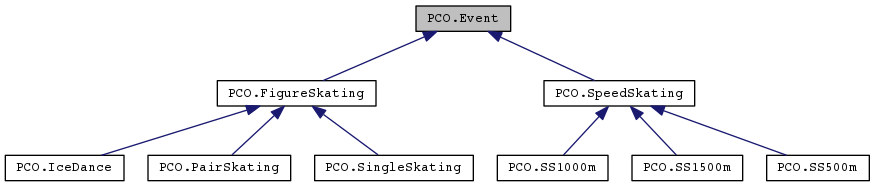
\includegraphics[width=350pt]{classPCO_1_1Event__inherit__graph}
\end{center}
\end{figure}
\subsection*{Classes}
\begin{DoxyCompactItemize}
\item 
interface \hyperlink{interfacePCO_1_1Event_1_1eventInheritance}{event\+Inheritance}
\end{DoxyCompactItemize}
\subsection*{Public Member Functions}
\begin{DoxyCompactItemize}
\item 
\hyperlink{classPCO_1_1Event_a55055f951cbfc76c9d62086b25aa93d0}{Event} ()
\item 
abstract int \hyperlink{classPCO_1_1Event_a89e26f29f5cfc92627bbb5a5e4ca1053}{event\+Num} ()
\item 
abstract void \hyperlink{classPCO_1_1Event_ad47d86904767dfebc731be328ec0958d}{run\+Event} (List$<$ \hyperlink{classPCO_1_1Judge}{Judge} $>$ j, List$<$ \hyperlink{classPCO_1_1Team}{Team} $>$ t)
\item 
abstract void \hyperlink{classPCO_1_1Event_a6a19f71e79d0f498ba74c9cd86c27eaa}{sched\+Event} (List$<$ \hyperlink{classPCO_1_1Judge}{Judge} $>$ j, List$<$ \hyperlink{classPCO_1_1Team}{Team} $>$ t)
\end{DoxyCompactItemize}


\subsection{Detailed Description}
\hyperlink{classPCO_1_1Event}{Event} class is the superclass of all the 2 event types and 6 specific events. 

D\+E\+F\+I\+N\+I\+T\+I\+O\+N\+: The specific competition at a specified rink determined by the schedule.

C\+O\+N\+S\+T\+R\+A\+I\+N\+T\+S\+: Limited to the six official events of the Winter Olympics. Events will not disturb those who are not registered for that specific event. Expunges the highest and lowest scores an individual or pair receives. Total score is the average of the remaining judges scores. Timed events utilize time as the score which a judge verifies.\begin{DoxyAuthor}{Author}
Landen Marchand 
\end{DoxyAuthor}


Definition at line 17 of file Event.\+cs.



\subsection{Constructor \& Destructor Documentation}
\hypertarget{classPCO_1_1Event_a55055f951cbfc76c9d62086b25aa93d0}{\index{P\+C\+O\+::\+Event@{P\+C\+O\+::\+Event}!Event@{Event}}
\index{Event@{Event}!P\+C\+O\+::\+Event@{P\+C\+O\+::\+Event}}
\subsubsection[{Event}]{\setlength{\rightskip}{0pt plus 5cm}P\+C\+O.\+Event.\+Event (
\begin{DoxyParamCaption}
{}
\end{DoxyParamCaption}
)\hspace{0.3cm}{\ttfamily [inline]}}}\label{classPCO_1_1Event_a55055f951cbfc76c9d62086b25aa93d0}
Default Constructor Provided Automatically 
\begin{DoxyParams}{Parameters}
{\em None} & \\
\hline
\end{DoxyParams}
\begin{DoxyReturn}{Returns}
Default Values 
\end{DoxyReturn}


Definition at line 23 of file Event.\+cs.



\subsection{Member Function Documentation}
\hypertarget{classPCO_1_1Event_a89e26f29f5cfc92627bbb5a5e4ca1053}{\index{P\+C\+O\+::\+Event@{P\+C\+O\+::\+Event}!event\+Num@{event\+Num}}
\index{event\+Num@{event\+Num}!P\+C\+O\+::\+Event@{P\+C\+O\+::\+Event}}
\subsubsection[{event\+Num}]{\setlength{\rightskip}{0pt plus 5cm}abstract int P\+C\+O.\+Event.\+event\+Num (
\begin{DoxyParamCaption}
{}
\end{DoxyParamCaption}
)\hspace{0.3cm}{\ttfamily [pure virtual]}}}\label{classPCO_1_1Event_a89e26f29f5cfc92627bbb5a5e4ca1053}
Inheritance member function for \hyperlink{classPCO_1_1SpeedSkating}{Speed\+Skating} and \hyperlink{classPCO_1_1FigureSkating}{Figure\+Skating} events Special identification number for unique event 
\begin{DoxyParams}{Parameters}
{\em none} & \\
\hline
\end{DoxyParams}
\begin{DoxyReturn}{Returns}
int pertaining to event I\+D 
\end{DoxyReturn}


Implemented in \hyperlink{classPCO_1_1IceDance_a4b5fe113cbbb0d2b59f97b58c3b15e79}{P\+C\+O.\+Ice\+Dance}, \hyperlink{classPCO_1_1PairSkating_aaf3cda572c411560ddc8f2f44621ff18}{P\+C\+O.\+Pair\+Skating}, \hyperlink{classPCO_1_1SingleSkating_ab7ac6446917e2d9fa363291ec473567d}{P\+C\+O.\+Single\+Skating}, \hyperlink{classPCO_1_1SS1000m_a7087df2094b075191b778e7b56ea07fd}{P\+C\+O.\+S\+S1000m}, \hyperlink{classPCO_1_1SS1500m_ab027d041adf7b8dea0b3189948ceb5d1}{P\+C\+O.\+S\+S1500m}, and \hyperlink{classPCO_1_1SS500m_a909b7bee200b907aae35d8bc47d442e5}{P\+C\+O.\+S\+S500m}.

\hypertarget{classPCO_1_1Event_ad47d86904767dfebc731be328ec0958d}{\index{P\+C\+O\+::\+Event@{P\+C\+O\+::\+Event}!run\+Event@{run\+Event}}
\index{run\+Event@{run\+Event}!P\+C\+O\+::\+Event@{P\+C\+O\+::\+Event}}
\subsubsection[{run\+Event}]{\setlength{\rightskip}{0pt plus 5cm}abstract void P\+C\+O.\+Event.\+run\+Event (
\begin{DoxyParamCaption}
\item[{List$<$ {\bf Judge} $>$}]{j, }
\item[{List$<$ {\bf Team} $>$}]{t}
\end{DoxyParamCaption}
)\hspace{0.3cm}{\ttfamily [pure virtual]}}}\label{classPCO_1_1Event_ad47d86904767dfebc731be328ec0958d}
Inheritance member function for \hyperlink{classPCO_1_1SpeedSkating}{Speed\+Skating} and \hyperlink{classPCO_1_1FigureSkating}{Figure\+Skating} events Judges/\+Teams to run specific event 
\begin{DoxyParams}{Parameters}
{\em List$<$\+Judge$>$} & List of judges for event \\
\hline
{\em List$<$\+Team$>$} & List of teams for event \\
\hline
\end{DoxyParams}
\begin{DoxyReturn}{Returns}
none 
\end{DoxyReturn}


Implemented in \hyperlink{classPCO_1_1IceDance_ace6551516fc450a992074dacaff19294}{P\+C\+O.\+Ice\+Dance}, \hyperlink{classPCO_1_1PairSkating_adc75a58b22ce9edd905cbbe06320c9a1}{P\+C\+O.\+Pair\+Skating}, \hyperlink{classPCO_1_1SingleSkating_aae06189e3102d74a26b7af29338a168a}{P\+C\+O.\+Single\+Skating}, \hyperlink{classPCO_1_1SS1000m_a00263d1777d343e9485a0da0e5e7f910}{P\+C\+O.\+S\+S1000m}, \hyperlink{classPCO_1_1SS1500m_a2e52ec9781aedcfdf1a47d8a8f4560ff}{P\+C\+O.\+S\+S1500m}, and \hyperlink{classPCO_1_1SS500m_a3ebc360a0ec5c60e1d2c66511c8f8025}{P\+C\+O.\+S\+S500m}.

\hypertarget{classPCO_1_1Event_a6a19f71e79d0f498ba74c9cd86c27eaa}{\index{P\+C\+O\+::\+Event@{P\+C\+O\+::\+Event}!sched\+Event@{sched\+Event}}
\index{sched\+Event@{sched\+Event}!P\+C\+O\+::\+Event@{P\+C\+O\+::\+Event}}
\subsubsection[{sched\+Event}]{\setlength{\rightskip}{0pt plus 5cm}abstract void P\+C\+O.\+Event.\+sched\+Event (
\begin{DoxyParamCaption}
\item[{List$<$ {\bf Judge} $>$}]{j, }
\item[{List$<$ {\bf Team} $>$}]{t}
\end{DoxyParamCaption}
)\hspace{0.3cm}{\ttfamily [pure virtual]}}}\label{classPCO_1_1Event_a6a19f71e79d0f498ba74c9cd86c27eaa}
Inheritance member function for \hyperlink{classPCO_1_1SpeedSkating}{Speed\+Skating} and \hyperlink{classPCO_1_1FigureSkating}{Figure\+Skating} events Juges/\+Teams to be scheduled for future events 
\begin{DoxyParams}{Parameters}
{\em List$<$\+Judge$>$} & List of judges for event \\
\hline
{\em List$<$\+Team$>$} & List of teams for event \\
\hline
\end{DoxyParams}
\begin{DoxyReturn}{Returns}
none 
\end{DoxyReturn}


Implemented in \hyperlink{classPCO_1_1IceDance_a60f5dea6597535a8b06baed8d71a27e1}{P\+C\+O.\+Ice\+Dance}, \hyperlink{classPCO_1_1PairSkating_a7da01fe6e5c700bc232189087fddf450}{P\+C\+O.\+Pair\+Skating}, \hyperlink{classPCO_1_1SingleSkating_ae97935dfac37a5818431c5b9de138345}{P\+C\+O.\+Single\+Skating}, \hyperlink{classPCO_1_1SS1000m_a883e286f1896171885422cf5c143c2da}{P\+C\+O.\+S\+S1000m}, \hyperlink{classPCO_1_1SS1500m_aebbf1e9bd3d845f68339381daf22ef23}{P\+C\+O.\+S\+S1500m}, and \hyperlink{classPCO_1_1SS500m_a760bbe2b60121e4fe86c64f2c8b60848}{P\+C\+O.\+S\+S500m}.



The documentation for this class was generated from the following file\+:\begin{DoxyCompactItemize}
\item 
\hyperlink{Event_8cs}{Event.\+cs}\end{DoxyCompactItemize}

\hypertarget{classPCO_1_1FigureSkating}{\section{P\+C\+O.\+Figure\+Skating Class Reference}
\label{classPCO_1_1FigureSkating}\index{P\+C\+O.\+Figure\+Skating@{P\+C\+O.\+Figure\+Skating}}
}


\hyperlink{classPCO_1_1FigureSkating}{Figure\+Skating} class is the superclass of the 3 \hyperlink{classPCO_1_1FigureSkating}{Figure\+Skating} events.  




Inheritance diagram for P\+C\+O.\+Figure\+Skating\+:\nopagebreak
\begin{figure}[H]
\begin{center}
\leavevmode
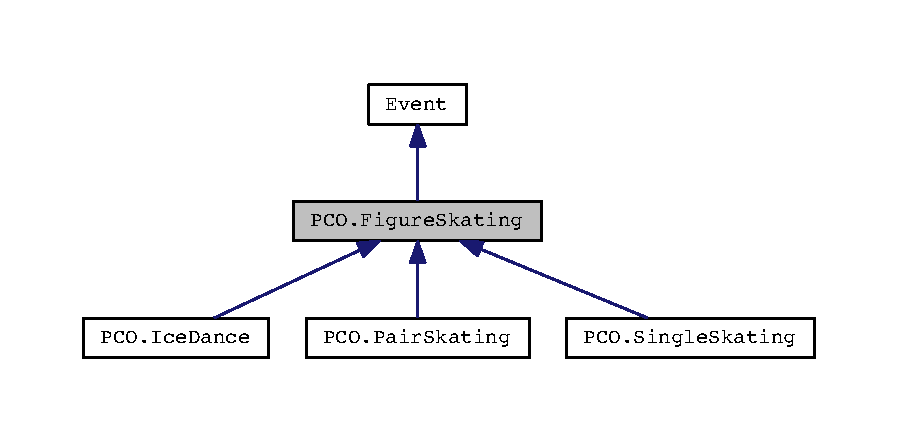
\includegraphics[width=350pt]{classPCO_1_1FigureSkating__inherit__graph}
\end{center}
\end{figure}


Collaboration diagram for P\+C\+O.\+Figure\+Skating\+:\nopagebreak
\begin{figure}[H]
\begin{center}
\leavevmode
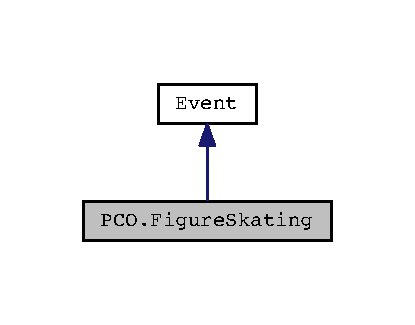
\includegraphics[width=199pt]{classPCO_1_1FigureSkating__coll__graph}
\end{center}
\end{figure}
\subsection*{Classes}
\begin{DoxyCompactItemize}
\item 
interface \hyperlink{interfacePCO_1_1FigureSkating_1_1ssInheritance}{ss\+Inheritance}
\end{DoxyCompactItemize}
\subsection*{Public Member Functions}
\begin{DoxyCompactItemize}
\item 
\hyperlink{classPCO_1_1FigureSkating_af988e41fae7e28d2b1a46c9c114726fd}{Figure\+Skating} ()
\item 
abstract double \hyperlink{classPCO_1_1FigureSkating_a5e2227ce9d5d0d49b295e48c7f43e88d}{fs\+Score} ()
\end{DoxyCompactItemize}
\subsection*{Additional Inherited Members}


\subsection{Detailed Description}
\hyperlink{classPCO_1_1FigureSkating}{Figure\+Skating} class is the superclass of the 3 \hyperlink{classPCO_1_1FigureSkating}{Figure\+Skating} events. 

D\+E\+F\+I\+N\+I\+T\+I\+O\+N\+: Skating done on ice in synchronization with music that is scored based upon technical tricks and or the synchronization of each athlete in a pair. One of the two main sporting categories that consist of three unique events which athletes participate separately as well as in pairs.

C\+O\+N\+S\+T\+R\+A\+I\+N\+T\+S\+: None\begin{DoxyAuthor}{Author}
Landen Marchand 
\end{DoxyAuthor}


Definition at line 16 of file Figure\+Skating.\+cs.



\subsection{Constructor \& Destructor Documentation}
\hypertarget{classPCO_1_1FigureSkating_af988e41fae7e28d2b1a46c9c114726fd}{\index{P\+C\+O\+::\+Figure\+Skating@{P\+C\+O\+::\+Figure\+Skating}!Figure\+Skating@{Figure\+Skating}}
\index{Figure\+Skating@{Figure\+Skating}!P\+C\+O\+::\+Figure\+Skating@{P\+C\+O\+::\+Figure\+Skating}}
\subsubsection[{Figure\+Skating}]{\setlength{\rightskip}{0pt plus 5cm}P\+C\+O.\+Figure\+Skating.\+Figure\+Skating (
\begin{DoxyParamCaption}
{}
\end{DoxyParamCaption}
)\hspace{0.3cm}{\ttfamily [inline]}}}\label{classPCO_1_1FigureSkating_af988e41fae7e28d2b1a46c9c114726fd}
Default Constructor Provided Automatically 
\begin{DoxyParams}{Parameters}
{\em None} & \\
\hline
\end{DoxyParams}
\begin{DoxyReturn}{Returns}
Default Values 
\end{DoxyReturn}


Definition at line 22 of file Figure\+Skating.\+cs.



\subsection{Member Function Documentation}
\hypertarget{classPCO_1_1FigureSkating_a5e2227ce9d5d0d49b295e48c7f43e88d}{\index{P\+C\+O\+::\+Figure\+Skating@{P\+C\+O\+::\+Figure\+Skating}!fs\+Score@{fs\+Score}}
\index{fs\+Score@{fs\+Score}!P\+C\+O\+::\+Figure\+Skating@{P\+C\+O\+::\+Figure\+Skating}}
\subsubsection[{fs\+Score}]{\setlength{\rightskip}{0pt plus 5cm}abstract double P\+C\+O.\+Figure\+Skating.\+fs\+Score (
\begin{DoxyParamCaption}
{}
\end{DoxyParamCaption}
)\hspace{0.3cm}{\ttfamily [pure virtual]}}}\label{classPCO_1_1FigureSkating_a5e2227ce9d5d0d49b295e48c7f43e88d}
Inheritance member function for \hyperlink{classPCO_1_1FigureSkating}{Figure\+Skating} events 
\begin{DoxyParams}{Parameters}
{\em none} & \\
\hline
\end{DoxyParams}
\begin{DoxyReturn}{Returns}
double pertaining to scores (completion of event of athlete) 
\end{DoxyReturn}


Implemented in \hyperlink{classPCO_1_1IceDance_a277430a17d25085022ea3567a133fa81}{P\+C\+O.\+Ice\+Dance}, \hyperlink{classPCO_1_1PairSkating_aaab23d1dec6f01ef77ec808be48d6b75}{P\+C\+O.\+Pair\+Skating}, and \hyperlink{classPCO_1_1SingleSkating_a36f8a341cc9e3259d898eb4ff15a98ec}{P\+C\+O.\+Single\+Skating}.



The documentation for this class was generated from the following file\+:\begin{DoxyCompactItemize}
\item 
\hyperlink{FigureSkating_8cs}{Figure\+Skating.\+cs}\end{DoxyCompactItemize}

\hypertarget{classPCO_1_1IceDance}{\section{P\+C\+O.\+Ice\+Dance Class Reference}
\label{classPCO_1_1IceDance}\index{P\+C\+O.\+Ice\+Dance@{P\+C\+O.\+Ice\+Dance}}
}


\hyperlink{classPCO_1_1IceDance}{Ice\+Dance} class is one of the 3 \hyperlink{classPCO_1_1FigureSkating}{Figure\+Skating} events.  




Inheritance diagram for P\+C\+O.\+Ice\+Dance\+:\nopagebreak
\begin{figure}[H]
\begin{center}
\leavevmode
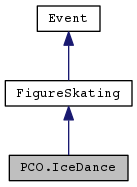
\includegraphics[width=175pt]{classPCO_1_1IceDance__inherit__graph}
\end{center}
\end{figure}


Collaboration diagram for P\+C\+O.\+Ice\+Dance\+:\nopagebreak
\begin{figure}[H]
\begin{center}
\leavevmode
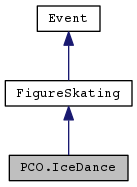
\includegraphics[width=175pt]{classPCO_1_1IceDance__coll__graph}
\end{center}
\end{figure}
\subsection*{Public Member Functions}
\begin{DoxyCompactItemize}
\item 
\hyperlink{classPCO_1_1IceDance_af8e9012b4a272fc2338c009dc25a5080}{Ice\+Dance} ()
\item 
override double \hyperlink{classPCO_1_1IceDance_a277430a17d25085022ea3567a133fa81}{fs\+Score} ()
\item 
override int \hyperlink{classPCO_1_1IceDance_a4b5fe113cbbb0d2b59f97b58c3b15e79}{event\+Num} ()
\item 
override void \hyperlink{classPCO_1_1IceDance_ace6551516fc450a992074dacaff19294}{run\+Event} (List$<$ \hyperlink{classPCO_1_1Judge}{Judge} $>$ j, List$<$ \hyperlink{classPCO_1_1Team}{Team} $>$ t)
\item 
override void \hyperlink{classPCO_1_1IceDance_a60f5dea6597535a8b06baed8d71a27e1}{sched\+Event} (List$<$ \hyperlink{classPCO_1_1Judge}{Judge} $>$ j, List$<$ \hyperlink{classPCO_1_1Team}{Team} $>$ t)
\end{DoxyCompactItemize}


\subsection{Detailed Description}
\hyperlink{classPCO_1_1IceDance}{Ice\+Dance} class is one of the 3 \hyperlink{classPCO_1_1FigureSkating}{Figure\+Skating} events. 

D\+E\+F\+I\+N\+I\+T\+I\+O\+N\+: Form of figure skating where athletes participate in male/female pairs. The utilization of the same technique as Pair Skating is present but the dancing is all done in tandem versus implementing technical tricks.

C\+O\+N\+S\+T\+R\+A\+I\+N\+T\+S\+: The pairs are male/female. Each pair performs solo on the rink at a given time. Total duration of performance is 4 mintues and 30 seconds.\begin{DoxyAuthor}{Author}
Landen Marchand 
\end{DoxyAuthor}


Definition at line 17 of file Ice\+Dance.\+cs.



\subsection{Constructor \& Destructor Documentation}
\hypertarget{classPCO_1_1IceDance_af8e9012b4a272fc2338c009dc25a5080}{\index{P\+C\+O\+::\+Ice\+Dance@{P\+C\+O\+::\+Ice\+Dance}!Ice\+Dance@{Ice\+Dance}}
\index{Ice\+Dance@{Ice\+Dance}!P\+C\+O\+::\+Ice\+Dance@{P\+C\+O\+::\+Ice\+Dance}}
\subsubsection[{Ice\+Dance}]{\setlength{\rightskip}{0pt plus 5cm}P\+C\+O.\+Ice\+Dance.\+Ice\+Dance (
\begin{DoxyParamCaption}
{}
\end{DoxyParamCaption}
)\hspace{0.3cm}{\ttfamily [inline]}}}\label{classPCO_1_1IceDance_af8e9012b4a272fc2338c009dc25a5080}
Default Constructor Provided Automatically 
\begin{DoxyParams}{Parameters}
{\em None} & \\
\hline
\end{DoxyParams}
\begin{DoxyReturn}{Returns}
Default Values 
\end{DoxyReturn}


Definition at line 23 of file Ice\+Dance.\+cs.



\subsection{Member Function Documentation}
\hypertarget{classPCO_1_1IceDance_a4b5fe113cbbb0d2b59f97b58c3b15e79}{\index{P\+C\+O\+::\+Ice\+Dance@{P\+C\+O\+::\+Ice\+Dance}!event\+Num@{event\+Num}}
\index{event\+Num@{event\+Num}!P\+C\+O\+::\+Ice\+Dance@{P\+C\+O\+::\+Ice\+Dance}}
\subsubsection[{event\+Num}]{\setlength{\rightskip}{0pt plus 5cm}override int P\+C\+O.\+Ice\+Dance.\+event\+Num (
\begin{DoxyParamCaption}
{}
\end{DoxyParamCaption}
)\hspace{0.3cm}{\ttfamily [inline]}, {\ttfamily [virtual]}}}\label{classPCO_1_1IceDance_a4b5fe113cbbb0d2b59f97b58c3b15e79}
Function to override inherited \hyperlink{classPCO_1_1IceDance_a4b5fe113cbbb0d2b59f97b58c3b15e79}{event\+Num()} function 

Implements \hyperlink{classPCO_1_1Event_a89e26f29f5cfc92627bbb5a5e4ca1053}{P\+C\+O.\+Event}.



Definition at line 34 of file Ice\+Dance.\+cs.

\hypertarget{classPCO_1_1IceDance_a277430a17d25085022ea3567a133fa81}{\index{P\+C\+O\+::\+Ice\+Dance@{P\+C\+O\+::\+Ice\+Dance}!fs\+Score@{fs\+Score}}
\index{fs\+Score@{fs\+Score}!P\+C\+O\+::\+Ice\+Dance@{P\+C\+O\+::\+Ice\+Dance}}
\subsubsection[{fs\+Score}]{\setlength{\rightskip}{0pt plus 5cm}override double P\+C\+O.\+Ice\+Dance.\+fs\+Score (
\begin{DoxyParamCaption}
{}
\end{DoxyParamCaption}
)\hspace{0.3cm}{\ttfamily [inline]}, {\ttfamily [virtual]}}}\label{classPCO_1_1IceDance_a277430a17d25085022ea3567a133fa81}
Function to override inherited \hyperlink{classPCO_1_1IceDance_a277430a17d25085022ea3567a133fa81}{fs\+Score()} function 

Implements \hyperlink{classPCO_1_1FigureSkating_a5e2227ce9d5d0d49b295e48c7f43e88d}{P\+C\+O.\+Figure\+Skating}.



Definition at line 28 of file Ice\+Dance.\+cs.

\hypertarget{classPCO_1_1IceDance_ace6551516fc450a992074dacaff19294}{\index{P\+C\+O\+::\+Ice\+Dance@{P\+C\+O\+::\+Ice\+Dance}!run\+Event@{run\+Event}}
\index{run\+Event@{run\+Event}!P\+C\+O\+::\+Ice\+Dance@{P\+C\+O\+::\+Ice\+Dance}}
\subsubsection[{run\+Event}]{\setlength{\rightskip}{0pt plus 5cm}override void P\+C\+O.\+Ice\+Dance.\+run\+Event (
\begin{DoxyParamCaption}
\item[{List$<$ {\bf Judge} $>$}]{j, }
\item[{List$<$ {\bf Team} $>$}]{t}
\end{DoxyParamCaption}
)\hspace{0.3cm}{\ttfamily [inline]}, {\ttfamily [virtual]}}}\label{classPCO_1_1IceDance_ace6551516fc450a992074dacaff19294}
Function to override inherited run\+Event(..) function 

Implements \hyperlink{classPCO_1_1Event_ad47d86904767dfebc731be328ec0958d}{P\+C\+O.\+Event}.



Definition at line 40 of file Ice\+Dance.\+cs.

\hypertarget{classPCO_1_1IceDance_a60f5dea6597535a8b06baed8d71a27e1}{\index{P\+C\+O\+::\+Ice\+Dance@{P\+C\+O\+::\+Ice\+Dance}!sched\+Event@{sched\+Event}}
\index{sched\+Event@{sched\+Event}!P\+C\+O\+::\+Ice\+Dance@{P\+C\+O\+::\+Ice\+Dance}}
\subsubsection[{sched\+Event}]{\setlength{\rightskip}{0pt plus 5cm}override void P\+C\+O.\+Ice\+Dance.\+sched\+Event (
\begin{DoxyParamCaption}
\item[{List$<$ {\bf Judge} $>$}]{j, }
\item[{List$<$ {\bf Team} $>$}]{t}
\end{DoxyParamCaption}
)\hspace{0.3cm}{\ttfamily [inline]}, {\ttfamily [virtual]}}}\label{classPCO_1_1IceDance_a60f5dea6597535a8b06baed8d71a27e1}
Function to override inherited sched\+Event(..) function 

Implements \hyperlink{classPCO_1_1Event_a6a19f71e79d0f498ba74c9cd86c27eaa}{P\+C\+O.\+Event}.



Definition at line 46 of file Ice\+Dance.\+cs.



The documentation for this class was generated from the following file\+:\begin{DoxyCompactItemize}
\item 
\hyperlink{IceDance_8cs}{Ice\+Dance.\+cs}\end{DoxyCompactItemize}

\hypertarget{classPCO_1_1Judge}{\section{P\+C\+O.\+Judge Class Reference}
\label{classPCO_1_1Judge}\index{P\+C\+O.\+Judge@{P\+C\+O.\+Judge}}
}


\hyperlink{classPCO_1_1Judge}{Judge} class houses and disperses all the qualified judges.  


\subsection*{Public Member Functions}
\begin{DoxyCompactItemize}
\item 
\hyperlink{classPCO_1_1Judge_a6739597d9c654fc3609d0d446288aff9}{Judge} ()
\end{DoxyCompactItemize}
\subsection*{Properties}
\begin{DoxyCompactItemize}
\item 
int \hyperlink{classPCO_1_1Judge_ae025be7243620fb90013477bc81bb6ad}{judge\+I\+D}\hspace{0.3cm}{\ttfamily  \mbox{[}get, set\mbox{]}}
\item 
\hyperlink{classPCO_1_1Schedule}{Schedule} \hyperlink{classPCO_1_1Judge_abc1631a408c0d72e62daa23783cc6330}{judge\+Schedule}\hspace{0.3cm}{\ttfamily  \mbox{[}get, set\mbox{]}}
\item 
\hyperlink{classPCO_1_1Scoring}{Scoring} \hyperlink{classPCO_1_1Judge_a76d950e6f90615fe320c12db369da4c4}{judge\+Score}\hspace{0.3cm}{\ttfamily  \mbox{[}get, set\mbox{]}}
\end{DoxyCompactItemize}


\subsection{Detailed Description}
\hyperlink{classPCO_1_1Judge}{Judge} class houses and disperses all the qualified judges. 

D\+E\+F\+I\+N\+T\+I\+O\+N\+: A qualified person to score and assess each event. A judge is independent of all teams and free of any bias.

C\+O\+N\+S\+T\+R\+A\+I\+N\+T\+S\+: Provides a score ranging from 0 through 100 on scored events. Verifies accurate timing on timed events. Remains corruption-\/ free and has no contact with athletes.\begin{DoxyAuthor}{Author}
Landen Marchand 
\end{DoxyAuthor}


Definition at line 16 of file Judge.\+cs.



\subsection{Constructor \& Destructor Documentation}
\hypertarget{classPCO_1_1Judge_a6739597d9c654fc3609d0d446288aff9}{\index{P\+C\+O\+::\+Judge@{P\+C\+O\+::\+Judge}!Judge@{Judge}}
\index{Judge@{Judge}!P\+C\+O\+::\+Judge@{P\+C\+O\+::\+Judge}}
\subsubsection[{Judge}]{\setlength{\rightskip}{0pt plus 5cm}P\+C\+O.\+Judge.\+Judge (
\begin{DoxyParamCaption}
{}
\end{DoxyParamCaption}
)\hspace{0.3cm}{\ttfamily [inline]}}}\label{classPCO_1_1Judge_a6739597d9c654fc3609d0d446288aff9}
Default Constructor Provided Automatically 
\begin{DoxyParams}{Parameters}
{\em None} & \\
\hline
\end{DoxyParams}
\begin{DoxyReturn}{Returns}
Default Values 
\end{DoxyReturn}


Definition at line 22 of file Judge.\+cs.



\subsection{Property Documentation}
\hypertarget{classPCO_1_1Judge_ae025be7243620fb90013477bc81bb6ad}{\index{P\+C\+O\+::\+Judge@{P\+C\+O\+::\+Judge}!judge\+I\+D@{judge\+I\+D}}
\index{judge\+I\+D@{judge\+I\+D}!P\+C\+O\+::\+Judge@{P\+C\+O\+::\+Judge}}
\subsubsection[{judge\+I\+D}]{\setlength{\rightskip}{0pt plus 5cm}int P\+C\+O.\+Judge.\+judge\+I\+D\hspace{0.3cm}{\ttfamily [get]}, {\ttfamily [set]}}}\label{classPCO_1_1Judge_ae025be7243620fb90013477bc81bb6ad}
Sets and gets judge's I\+D number 
\begin{DoxyParams}{Parameters}
{\em int} & for I\+D number \\
\hline
\end{DoxyParams}
\begin{DoxyReturn}{Returns}
int I\+D number 
\end{DoxyReturn}


Definition at line 29 of file Judge.\+cs.

\hypertarget{classPCO_1_1Judge_abc1631a408c0d72e62daa23783cc6330}{\index{P\+C\+O\+::\+Judge@{P\+C\+O\+::\+Judge}!judge\+Schedule@{judge\+Schedule}}
\index{judge\+Schedule@{judge\+Schedule}!P\+C\+O\+::\+Judge@{P\+C\+O\+::\+Judge}}
\subsubsection[{judge\+Schedule}]{\setlength{\rightskip}{0pt plus 5cm}{\bf Schedule} P\+C\+O.\+Judge.\+judge\+Schedule\hspace{0.3cm}{\ttfamily [get]}, {\ttfamily [set]}}}\label{classPCO_1_1Judge_abc1631a408c0d72e62daa23783cc6330}
Sets and gets the schedule for each judge 
\begin{DoxyParams}{Parameters}
{\em \hyperlink{classPCO_1_1Schedule}{Schedule}} & \\
\hline
\end{DoxyParams}
\begin{DoxyReturn}{Returns}
\hyperlink{classPCO_1_1Schedule}{Schedule} 
\end{DoxyReturn}


Definition at line 34 of file Judge.\+cs.

\hypertarget{classPCO_1_1Judge_a76d950e6f90615fe320c12db369da4c4}{\index{P\+C\+O\+::\+Judge@{P\+C\+O\+::\+Judge}!judge\+Score@{judge\+Score}}
\index{judge\+Score@{judge\+Score}!P\+C\+O\+::\+Judge@{P\+C\+O\+::\+Judge}}
\subsubsection[{judge\+Score}]{\setlength{\rightskip}{0pt plus 5cm}{\bf Scoring} P\+C\+O.\+Judge.\+judge\+Score\hspace{0.3cm}{\ttfamily [get]}, {\ttfamily [set]}}}\label{classPCO_1_1Judge_a76d950e6f90615fe320c12db369da4c4}
Sets and gets the score for each event 
\begin{DoxyParams}{Parameters}
{\em \hyperlink{classPCO_1_1Scoring}{Scoring}} & \\
\hline
\end{DoxyParams}
\begin{DoxyReturn}{Returns}
\hyperlink{classPCO_1_1Scoring}{Scoring} 
\end{DoxyReturn}


Definition at line 39 of file Judge.\+cs.



The documentation for this class was generated from the following file\+:\begin{DoxyCompactItemize}
\item 
\hyperlink{Judge_8cs}{Judge.\+cs}\end{DoxyCompactItemize}

\hypertarget{classPCO_1_1MainClass}{\section{P\+C\+O.\+Main\+Class Class Reference}
\label{classPCO_1_1MainClass}\index{P\+C\+O.\+Main\+Class@{P\+C\+O.\+Main\+Class}}
}
\subsection*{Static Public Member Functions}
\begin{DoxyCompactItemize}
\item 
static void \hyperlink{classPCO_1_1MainClass_a48a102c6db73c0a2c03db47b91fb7f00}{Main} (string\mbox{[}$\,$\mbox{]} args)
\end{DoxyCompactItemize}


\subsection{Member Function Documentation}
\hypertarget{classPCO_1_1MainClass_a48a102c6db73c0a2c03db47b91fb7f00}{\index{P\+C\+O\+::\+Main\+Class@{P\+C\+O\+::\+Main\+Class}!Main@{Main}}
\index{Main@{Main}!P\+C\+O\+::\+Main\+Class@{P\+C\+O\+::\+Main\+Class}}
\subsubsection[{Main}]{\setlength{\rightskip}{0pt plus 5cm}static void P\+C\+O.\+Main\+Class.\+Main (
\begin{DoxyParamCaption}
\item[{string\mbox{[}$\,$\mbox{]}}]{args}
\end{DoxyParamCaption}
)\hspace{0.3cm}{\ttfamily [inline]}, {\ttfamily [static]}}}\label{classPCO_1_1MainClass_a48a102c6db73c0a2c03db47b91fb7f00}


The documentation for this class was generated from the following file\+:\begin{DoxyCompactItemize}
\item 
\hyperlink{Program_8cs}{Program.\+cs}\end{DoxyCompactItemize}

\hypertarget{classPCO_1_1PairSkating}{\section{P\+C\+O.\+Pair\+Skating Class Reference}
\label{classPCO_1_1PairSkating}\index{P\+C\+O.\+Pair\+Skating@{P\+C\+O.\+Pair\+Skating}}
}


\hyperlink{classPCO_1_1PairSkating}{Pair\+Skating} class is one of the 3 \hyperlink{classPCO_1_1FigureSkating}{Figure\+Skating} events.  




Inheritance diagram for P\+C\+O.\+Pair\+Skating\+:\nopagebreak
\begin{figure}[H]
\begin{center}
\leavevmode
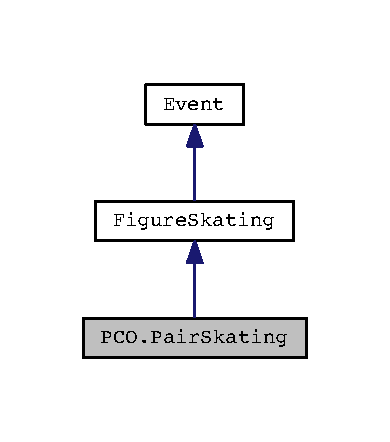
\includegraphics[width=187pt]{classPCO_1_1PairSkating__inherit__graph}
\end{center}
\end{figure}


Collaboration diagram for P\+C\+O.\+Pair\+Skating\+:\nopagebreak
\begin{figure}[H]
\begin{center}
\leavevmode
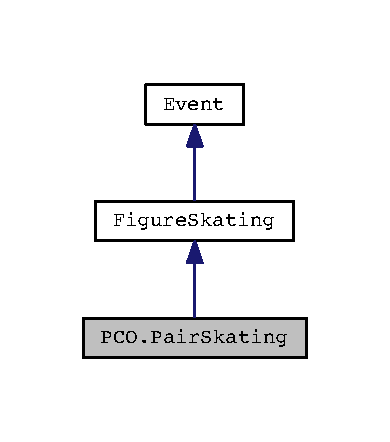
\includegraphics[width=187pt]{classPCO_1_1PairSkating__coll__graph}
\end{center}
\end{figure}
\subsection*{Public Member Functions}
\begin{DoxyCompactItemize}
\item 
\hyperlink{classPCO_1_1PairSkating_afcb237a5c3a41d42ebe8902b5ef2a4ec}{Pair\+Skating} ()
\item 
override double \hyperlink{classPCO_1_1PairSkating_aaab23d1dec6f01ef77ec808be48d6b75}{fs\+Score} ()
\item 
override int \hyperlink{classPCO_1_1PairSkating_aaf3cda572c411560ddc8f2f44621ff18}{event\+Num} ()
\item 
override void \hyperlink{classPCO_1_1PairSkating_adc75a58b22ce9edd905cbbe06320c9a1}{run\+Event} (List$<$ \hyperlink{classPCO_1_1Judge}{Judge} $>$ j, List$<$ \hyperlink{classPCO_1_1Team}{Team} $>$ t)
\item 
override void \hyperlink{classPCO_1_1PairSkating_a7da01fe6e5c700bc232189087fddf450}{sched\+Event} (List$<$ \hyperlink{classPCO_1_1Judge}{Judge} $>$ j, List$<$ \hyperlink{classPCO_1_1Team}{Team} $>$ t)
\end{DoxyCompactItemize}
\subsection*{Additional Inherited Members}


\subsection{Detailed Description}
\hyperlink{classPCO_1_1PairSkating}{Pair\+Skating} class is one of the 3 \hyperlink{classPCO_1_1FigureSkating}{Figure\+Skating} events. 

D\+E\+F\+I\+N\+I\+T\+I\+O\+N\+: Form of figure skating where athletes participate in male/female pairs. The utilization of long program style where each athlete is free to do their own unique performance complete with technical tricks is present.

C\+O\+N\+S\+T\+R\+A\+I\+N\+T\+S\+: The pairs are male female. Each pair performs solo on the rink at a given time. Total duration of performance is 4 mintues and 30 seconds.\begin{DoxyAuthor}{Author}
Landen Marchand 
\end{DoxyAuthor}


Definition at line 17 of file Pair\+Skating.\+cs.



\subsection{Constructor \& Destructor Documentation}
\hypertarget{classPCO_1_1PairSkating_afcb237a5c3a41d42ebe8902b5ef2a4ec}{\index{P\+C\+O\+::\+Pair\+Skating@{P\+C\+O\+::\+Pair\+Skating}!Pair\+Skating@{Pair\+Skating}}
\index{Pair\+Skating@{Pair\+Skating}!P\+C\+O\+::\+Pair\+Skating@{P\+C\+O\+::\+Pair\+Skating}}
\subsubsection[{Pair\+Skating}]{\setlength{\rightskip}{0pt plus 5cm}P\+C\+O.\+Pair\+Skating.\+Pair\+Skating (
\begin{DoxyParamCaption}
{}
\end{DoxyParamCaption}
)\hspace{0.3cm}{\ttfamily [inline]}}}\label{classPCO_1_1PairSkating_afcb237a5c3a41d42ebe8902b5ef2a4ec}
Default Constructor Provided Automatically 
\begin{DoxyParams}{Parameters}
{\em None} & \\
\hline
\end{DoxyParams}
\begin{DoxyReturn}{Returns}
Default Values 
\end{DoxyReturn}


Definition at line 23 of file Pair\+Skating.\+cs.



\subsection{Member Function Documentation}
\hypertarget{classPCO_1_1PairSkating_aaf3cda572c411560ddc8f2f44621ff18}{\index{P\+C\+O\+::\+Pair\+Skating@{P\+C\+O\+::\+Pair\+Skating}!event\+Num@{event\+Num}}
\index{event\+Num@{event\+Num}!P\+C\+O\+::\+Pair\+Skating@{P\+C\+O\+::\+Pair\+Skating}}
\subsubsection[{event\+Num}]{\setlength{\rightskip}{0pt plus 5cm}override int P\+C\+O.\+Pair\+Skating.\+event\+Num (
\begin{DoxyParamCaption}
{}
\end{DoxyParamCaption}
)\hspace{0.3cm}{\ttfamily [inline]}, {\ttfamily [virtual]}}}\label{classPCO_1_1PairSkating_aaf3cda572c411560ddc8f2f44621ff18}
Function to override inherited \hyperlink{classPCO_1_1PairSkating_aaf3cda572c411560ddc8f2f44621ff18}{event\+Num()} function 

Implements \hyperlink{classPCO_1_1Event_a89e26f29f5cfc92627bbb5a5e4ca1053}{P\+C\+O.\+Event}.



Definition at line 34 of file Pair\+Skating.\+cs.

\hypertarget{classPCO_1_1PairSkating_aaab23d1dec6f01ef77ec808be48d6b75}{\index{P\+C\+O\+::\+Pair\+Skating@{P\+C\+O\+::\+Pair\+Skating}!fs\+Score@{fs\+Score}}
\index{fs\+Score@{fs\+Score}!P\+C\+O\+::\+Pair\+Skating@{P\+C\+O\+::\+Pair\+Skating}}
\subsubsection[{fs\+Score}]{\setlength{\rightskip}{0pt plus 5cm}override double P\+C\+O.\+Pair\+Skating.\+fs\+Score (
\begin{DoxyParamCaption}
{}
\end{DoxyParamCaption}
)\hspace{0.3cm}{\ttfamily [inline]}, {\ttfamily [virtual]}}}\label{classPCO_1_1PairSkating_aaab23d1dec6f01ef77ec808be48d6b75}
Function to override inherited \hyperlink{classPCO_1_1PairSkating_aaab23d1dec6f01ef77ec808be48d6b75}{fs\+Score()} function 

Implements \hyperlink{classPCO_1_1FigureSkating_a5e2227ce9d5d0d49b295e48c7f43e88d}{P\+C\+O.\+Figure\+Skating}.



Definition at line 28 of file Pair\+Skating.\+cs.

\hypertarget{classPCO_1_1PairSkating_adc75a58b22ce9edd905cbbe06320c9a1}{\index{P\+C\+O\+::\+Pair\+Skating@{P\+C\+O\+::\+Pair\+Skating}!run\+Event@{run\+Event}}
\index{run\+Event@{run\+Event}!P\+C\+O\+::\+Pair\+Skating@{P\+C\+O\+::\+Pair\+Skating}}
\subsubsection[{run\+Event}]{\setlength{\rightskip}{0pt plus 5cm}override void P\+C\+O.\+Pair\+Skating.\+run\+Event (
\begin{DoxyParamCaption}
\item[{List$<$ {\bf Judge} $>$}]{j, }
\item[{List$<$ {\bf Team} $>$}]{t}
\end{DoxyParamCaption}
)\hspace{0.3cm}{\ttfamily [inline]}, {\ttfamily [virtual]}}}\label{classPCO_1_1PairSkating_adc75a58b22ce9edd905cbbe06320c9a1}
Function to override inherited run\+Event(..) function 

Implements \hyperlink{classPCO_1_1Event_ad47d86904767dfebc731be328ec0958d}{P\+C\+O.\+Event}.



Definition at line 40 of file Pair\+Skating.\+cs.

\hypertarget{classPCO_1_1PairSkating_a7da01fe6e5c700bc232189087fddf450}{\index{P\+C\+O\+::\+Pair\+Skating@{P\+C\+O\+::\+Pair\+Skating}!sched\+Event@{sched\+Event}}
\index{sched\+Event@{sched\+Event}!P\+C\+O\+::\+Pair\+Skating@{P\+C\+O\+::\+Pair\+Skating}}
\subsubsection[{sched\+Event}]{\setlength{\rightskip}{0pt plus 5cm}override void P\+C\+O.\+Pair\+Skating.\+sched\+Event (
\begin{DoxyParamCaption}
\item[{List$<$ {\bf Judge} $>$}]{j, }
\item[{List$<$ {\bf Team} $>$}]{t}
\end{DoxyParamCaption}
)\hspace{0.3cm}{\ttfamily [inline]}, {\ttfamily [virtual]}}}\label{classPCO_1_1PairSkating_a7da01fe6e5c700bc232189087fddf450}
Function to override inherited sched\+Event(..) function 

Implements \hyperlink{classPCO_1_1Event_a6a19f71e79d0f498ba74c9cd86c27eaa}{P\+C\+O.\+Event}.



Definition at line 46 of file Pair\+Skating.\+cs.



The documentation for this class was generated from the following file\+:\begin{DoxyCompactItemize}
\item 
\hyperlink{PairSkating_8cs}{Pair\+Skating.\+cs}\end{DoxyCompactItemize}

\hypertarget{classPCO_1_1Registration}{\section{P\+C\+O.\+Registration Class Reference}
\label{classPCO_1_1Registration}\index{P\+C\+O.\+Registration@{P\+C\+O.\+Registration}}
}


\hyperlink{classPCO_1_1Registration}{Registration} class registers Teams and Athletes.  


\subsection*{Public Member Functions}
\begin{DoxyCompactItemize}
\item 
\hyperlink{classPCO_1_1Registration_a74519be4876c47630ca2b5f5084d48eb}{Registration} ()
\item 
List$<$ \hyperlink{classPCO_1_1Team}{Team} $>$ \hyperlink{classPCO_1_1Registration_ab5854210421c2f480d8a50bf87b4e739}{register\+Team} ()
\item 
List$<$ \hyperlink{classPCO_1_1Team}{Team} $>$ \hyperlink{classPCO_1_1Registration_ab574ad030f255cffd60cc6c2dbb0acea}{deregister\+Team} ()
\end{DoxyCompactItemize}


\subsection{Detailed Description}
\hyperlink{classPCO_1_1Registration}{Registration} class registers Teams and Athletes. 

D\+E\+F\+I\+N\+T\+I\+O\+N\+: The process of obtaining athletes who have successfully completed all qualification rounds prior to the Winter Olympics. \hyperlink{classPCO_1_1Registration}{Registration} places athletes into their respective team and places athletes to a specified event.

C\+O\+N\+S\+T\+R\+A\+I\+N\+T\+S\+: Sets a maximum limit of athletes per event. Sets a max limit on number of teams in the Winter Olympics.\begin{DoxyAuthor}{Author}
Landen Marchand 
\end{DoxyAuthor}


Definition at line 16 of file Registration.\+cs.



\subsection{Constructor \& Destructor Documentation}
\hypertarget{classPCO_1_1Registration_a74519be4876c47630ca2b5f5084d48eb}{\index{P\+C\+O\+::\+Registration@{P\+C\+O\+::\+Registration}!Registration@{Registration}}
\index{Registration@{Registration}!P\+C\+O\+::\+Registration@{P\+C\+O\+::\+Registration}}
\subsubsection[{Registration}]{\setlength{\rightskip}{0pt plus 5cm}P\+C\+O.\+Registration.\+Registration (
\begin{DoxyParamCaption}
{}
\end{DoxyParamCaption}
)\hspace{0.3cm}{\ttfamily [inline]}}}\label{classPCO_1_1Registration_a74519be4876c47630ca2b5f5084d48eb}
Default Constructor Provided Automatically 
\begin{DoxyParams}{Parameters}
{\em None} & \\
\hline
\end{DoxyParams}
\begin{DoxyReturn}{Returns}
Default Values 
\end{DoxyReturn}


Definition at line 22 of file Registration.\+cs.



\subsection{Member Function Documentation}
\hypertarget{classPCO_1_1Registration_ab574ad030f255cffd60cc6c2dbb0acea}{\index{P\+C\+O\+::\+Registration@{P\+C\+O\+::\+Registration}!deregister\+Team@{deregister\+Team}}
\index{deregister\+Team@{deregister\+Team}!P\+C\+O\+::\+Registration@{P\+C\+O\+::\+Registration}}
\subsubsection[{deregister\+Team}]{\setlength{\rightskip}{0pt plus 5cm}List$<${\bf Team}$>$ P\+C\+O.\+Registration.\+deregister\+Team (
\begin{DoxyParamCaption}
{}
\end{DoxyParamCaption}
)\hspace{0.3cm}{\ttfamily [inline]}}}\label{classPCO_1_1Registration_ab574ad030f255cffd60cc6c2dbb0acea}
Officially deregisteres an entire team from the Winter Olympics  $<$\+Team$>$ that is updated and contains one less team 

Definition at line 41 of file Registration.\+cs.

\hypertarget{classPCO_1_1Registration_ab5854210421c2f480d8a50bf87b4e739}{\index{P\+C\+O\+::\+Registration@{P\+C\+O\+::\+Registration}!register\+Team@{register\+Team}}
\index{register\+Team@{register\+Team}!P\+C\+O\+::\+Registration@{P\+C\+O\+::\+Registration}}
\subsubsection[{register\+Team}]{\setlength{\rightskip}{0pt plus 5cm}List$<${\bf Team}$>$ P\+C\+O.\+Registration.\+register\+Team (
\begin{DoxyParamCaption}
{}
\end{DoxyParamCaption}
)\hspace{0.3cm}{\ttfamily [inline]}}}\label{classPCO_1_1Registration_ab5854210421c2f480d8a50bf87b4e739}
Officially enters a team into the Winter Olympics $\ast$$\ast$\+N\+O\+T\+E\+: T\+H\+I\+S W\+I\+L\+L B\+E M\+O\+D\+I\+F\+I\+E\+D A\+F\+T\+E\+R M\+O\+R\+E I\+N\+F\+O I\+S O\+B\+T\+A\+I\+N\+E\+D$\ast$$\ast$ 
\begin{DoxyParams}{Parameters}
{\em none} & \\
\hline
\end{DoxyParams}
\begin{DoxyReturn}{Returns}
List$<$\+Team$>$ which is the official list of all teams and their athletes 
\end{DoxyReturn}


Definition at line 32 of file Registration.\+cs.



The documentation for this class was generated from the following file\+:\begin{DoxyCompactItemize}
\item 
\hyperlink{Registration_8cs}{Registration.\+cs}\end{DoxyCompactItemize}

\hypertarget{classPCO_1_1Rink}{\section{P\+C\+O.\+Rink Class Reference}
\label{classPCO_1_1Rink}\index{P\+C\+O.\+Rink@{P\+C\+O.\+Rink}}
}


\hyperlink{classPCO_1_1Rink}{Rink} class is the physical area in which events are held.  


\subsection*{Public Member Functions}
\begin{DoxyCompactItemize}
\item 
\hyperlink{classPCO_1_1Rink_ac0a83730147b9a04f26b0c41e5337be7}{Rink} ()
\item 
List$<$ \hyperlink{classPCO_1_1Event}{Event} $>$ \hyperlink{classPCO_1_1Rink_a683b279845f595abf88cc73f87e7f691}{rink\+Events} ()
\end{DoxyCompactItemize}


\subsection{Detailed Description}
\hyperlink{classPCO_1_1Rink}{Rink} class is the physical area in which events are held. 

D\+E\+F\+I\+N\+I\+T\+I\+O\+N\+: The location of each event determined by the schedule.

C\+O\+N\+S\+T\+R\+A\+I\+N\+T\+S\+: May only be occupied by one event at any given time. Must be in operation concurrent with the other rinks.\begin{DoxyAuthor}{Author}
Landen Marchand 
\end{DoxyAuthor}


Definition at line 14 of file Rink.\+cs.



\subsection{Constructor \& Destructor Documentation}
\hypertarget{classPCO_1_1Rink_ac0a83730147b9a04f26b0c41e5337be7}{\index{P\+C\+O\+::\+Rink@{P\+C\+O\+::\+Rink}!Rink@{Rink}}
\index{Rink@{Rink}!P\+C\+O\+::\+Rink@{P\+C\+O\+::\+Rink}}
\subsubsection[{Rink}]{\setlength{\rightskip}{0pt plus 5cm}P\+C\+O.\+Rink.\+Rink (
\begin{DoxyParamCaption}
{}
\end{DoxyParamCaption}
)\hspace{0.3cm}{\ttfamily [inline]}}}\label{classPCO_1_1Rink_ac0a83730147b9a04f26b0c41e5337be7}
Default Constructor Provided Automatically 
\begin{DoxyParams}{Parameters}
{\em None} & \\
\hline
\end{DoxyParams}
\begin{DoxyReturn}{Returns}
Default Values 
\end{DoxyReturn}


Definition at line 20 of file Rink.\+cs.



\subsection{Member Function Documentation}
\hypertarget{classPCO_1_1Rink_a683b279845f595abf88cc73f87e7f691}{\index{P\+C\+O\+::\+Rink@{P\+C\+O\+::\+Rink}!rink\+Events@{rink\+Events}}
\index{rink\+Events@{rink\+Events}!P\+C\+O\+::\+Rink@{P\+C\+O\+::\+Rink}}
\subsubsection[{rink\+Events}]{\setlength{\rightskip}{0pt plus 5cm}List$<${\bf Event}$>$ P\+C\+O.\+Rink.\+rink\+Events (
\begin{DoxyParamCaption}
{}
\end{DoxyParamCaption}
)\hspace{0.3cm}{\ttfamily [inline]}}}\label{classPCO_1_1Rink_a683b279845f595abf88cc73f87e7f691}
Function to obtain all the events that are held on a certain rink 
\begin{DoxyParams}{Parameters}
{\em none} & \\
\hline
\end{DoxyParams}
\begin{DoxyReturn}{Returns}
List$<$\+Event$>$ which is the list of all events that are held on a particular rink 
\end{DoxyReturn}


Definition at line 28 of file Rink.\+cs.



The documentation for this class was generated from the following file\+:\begin{DoxyCompactItemize}
\item 
\hyperlink{Rink_8cs}{Rink.\+cs}\end{DoxyCompactItemize}

\hypertarget{classPCO_1_1Schedule}{\section{P\+C\+O.\+Schedule Class Reference}
\label{classPCO_1_1Schedule}\index{P\+C\+O.\+Schedule@{P\+C\+O.\+Schedule}}
}


\hyperlink{classPCO_1_1Schedule}{Schedule} class is the organization of athletes and events.  


\subsection*{Public Member Functions}
\begin{DoxyCompactItemize}
\item 
\hyperlink{classPCO_1_1Schedule_ad35bec6c65e855eeb89793a4cafd8e6c}{Schedule} ()
\end{DoxyCompactItemize}


\subsection{Detailed Description}
\hyperlink{classPCO_1_1Schedule}{Schedule} class is the organization of athletes and events. 

D\+E\+F\+I\+N\+T\+I\+O\+N\+: The chronological listing of events over the course of two weeks. Scheduling implements where and when events are held. \hyperlink{classPCO_1_1Schedule}{Schedule} is also the organization of athletes placed into their respective events.

C\+O\+N\+S\+T\+R\+A\+I\+N\+T\+S\+: Must not organize events such that they happen concurrently on the same rink. Must not allot more than the appropriate amount of athletes per event. Must make sure any event is done as a pair contains one male and one female athlete per team.\begin{DoxyAuthor}{Author}
Landen Marchand 
\end{DoxyAuthor}


\subsection{Constructor \& Destructor Documentation}
\hypertarget{classPCO_1_1Schedule_ad35bec6c65e855eeb89793a4cafd8e6c}{\index{P\+C\+O\+::\+Schedule@{P\+C\+O\+::\+Schedule}!Schedule@{Schedule}}
\index{Schedule@{Schedule}!P\+C\+O\+::\+Schedule@{P\+C\+O\+::\+Schedule}}
\subsubsection[{Schedule}]{\setlength{\rightskip}{0pt plus 5cm}P\+C\+O.\+Schedule.\+Schedule (
\begin{DoxyParamCaption}
{}
\end{DoxyParamCaption}
)\hspace{0.3cm}{\ttfamily [inline]}}}\label{classPCO_1_1Schedule_ad35bec6c65e855eeb89793a4cafd8e6c}


The documentation for this class was generated from the following file\+:\begin{DoxyCompactItemize}
\item 
\hyperlink{Schedule_8cs}{Schedule.\+cs}\end{DoxyCompactItemize}

\hypertarget{classPCO_1_1Scoring}{\section{P\+C\+O.\+Scoring Class Reference}
\label{classPCO_1_1Scoring}\index{P\+C\+O.\+Scoring@{P\+C\+O.\+Scoring}}
}


\hyperlink{classPCO_1_1Scoring}{Scoring} class manages the official scores/times recorded by the judges.  


\subsection*{Public Member Functions}
\begin{DoxyCompactItemize}
\item 
\hyperlink{classPCO_1_1Scoring_a5c7b4dd99f9e1dd82da4a0e85442614f}{Scoring} ()
\end{DoxyCompactItemize}


\subsection{Detailed Description}
\hyperlink{classPCO_1_1Scoring}{Scoring} class manages the official scores/times recorded by the judges. 

D\+E\+F\+I\+N\+T\+I\+O\+N\+: The act of taking the judges scores that are given to the athlete or pair of athletes at their respective event.

C\+O\+N\+S\+T\+R\+A\+I\+N\+T\+S\+: Expunges the highest and lowest scores an individual or pair receives. Total score is the average of the remaining judges scores. Timed events utilize time as the score which a judge verifies.\begin{DoxyAuthor}{Author}
Landen Marchand 
\end{DoxyAuthor}


\subsection{Constructor \& Destructor Documentation}
\hypertarget{classPCO_1_1Scoring_a5c7b4dd99f9e1dd82da4a0e85442614f}{\index{P\+C\+O\+::\+Scoring@{P\+C\+O\+::\+Scoring}!Scoring@{Scoring}}
\index{Scoring@{Scoring}!P\+C\+O\+::\+Scoring@{P\+C\+O\+::\+Scoring}}
\subsubsection[{Scoring}]{\setlength{\rightskip}{0pt plus 5cm}P\+C\+O.\+Scoring.\+Scoring (
\begin{DoxyParamCaption}
{}
\end{DoxyParamCaption}
)\hspace{0.3cm}{\ttfamily [inline]}}}\label{classPCO_1_1Scoring_a5c7b4dd99f9e1dd82da4a0e85442614f}


The documentation for this class was generated from the following file\+:\begin{DoxyCompactItemize}
\item 
\hyperlink{Scoring_8cs}{Scoring.\+cs}\end{DoxyCompactItemize}

\hypertarget{classPCO_1_1SingleSkating}{\section{P\+C\+O.\+Single\+Skating Class Reference}
\label{classPCO_1_1SingleSkating}\index{P\+C\+O.\+Single\+Skating@{P\+C\+O.\+Single\+Skating}}
}


\hyperlink{classPCO_1_1SingleSkating}{Single\+Skating} class is one of the 3 \hyperlink{classPCO_1_1FigureSkating}{Figure\+Skating} events.  


\subsection*{Public Member Functions}
\begin{DoxyCompactItemize}
\item 
\hyperlink{classPCO_1_1SingleSkating_ae7c9d29f9cde56cd158564c20854f482}{Single\+Skating} ()
\end{DoxyCompactItemize}


\subsection{Detailed Description}
\hyperlink{classPCO_1_1SingleSkating}{Single\+Skating} class is one of the 3 \hyperlink{classPCO_1_1FigureSkating}{Figure\+Skating} events. 

D\+E\+F\+I\+N\+I\+T\+I\+O\+N\+: Form of figure skating where athletes participate individually. The utilization of long program style where each athlete is free to do their own unique performance complete with technical tricks is present.

C\+O\+N\+S\+T\+R\+A\+I\+N\+T\+S\+: Each athlete performs solo on the rink at a given time. Total duration of performance is 4 minutes and 30 seconds.\begin{DoxyAuthor}{Author}
Landen Marchand 
\end{DoxyAuthor}


\subsection{Constructor \& Destructor Documentation}
\hypertarget{classPCO_1_1SingleSkating_ae7c9d29f9cde56cd158564c20854f482}{\index{P\+C\+O\+::\+Single\+Skating@{P\+C\+O\+::\+Single\+Skating}!Single\+Skating@{Single\+Skating}}
\index{Single\+Skating@{Single\+Skating}!P\+C\+O\+::\+Single\+Skating@{P\+C\+O\+::\+Single\+Skating}}
\subsubsection[{Single\+Skating}]{\setlength{\rightskip}{0pt plus 5cm}P\+C\+O.\+Single\+Skating.\+Single\+Skating (
\begin{DoxyParamCaption}
{}
\end{DoxyParamCaption}
)\hspace{0.3cm}{\ttfamily [inline]}}}\label{classPCO_1_1SingleSkating_ae7c9d29f9cde56cd158564c20854f482}


The documentation for this class was generated from the following file\+:\begin{DoxyCompactItemize}
\item 
\hyperlink{SingleSkating_8cs}{Single\+Skating.\+cs}\end{DoxyCompactItemize}

\hypertarget{classPCO_1_1SpeedSkating}{\section{P\+C\+O.\+Speed\+Skating Class Reference}
\label{classPCO_1_1SpeedSkating}\index{P\+C\+O.\+Speed\+Skating@{P\+C\+O.\+Speed\+Skating}}
}


\hyperlink{classPCO_1_1SpeedSkating}{Speed\+Skating} class is the superclass of the 3 \hyperlink{classPCO_1_1SpeedSkating}{Speed\+Skating} events.  




Inheritance diagram for P\+C\+O.\+Speed\+Skating\+:\nopagebreak
\begin{figure}[H]
\begin{center}
\leavevmode
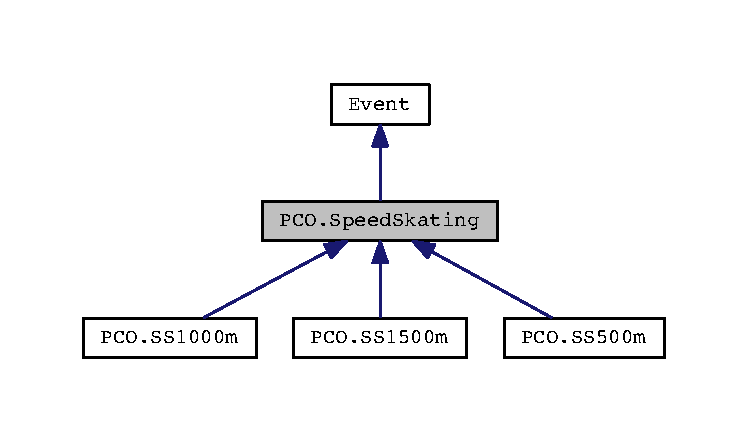
\includegraphics[width=350pt]{classPCO_1_1SpeedSkating__inherit__graph}
\end{center}
\end{figure}


Collaboration diagram for P\+C\+O.\+Speed\+Skating\+:\nopagebreak
\begin{figure}[H]
\begin{center}
\leavevmode
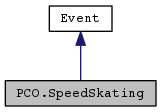
\includegraphics[width=193pt]{classPCO_1_1SpeedSkating__coll__graph}
\end{center}
\end{figure}
\subsection*{Classes}
\begin{DoxyCompactItemize}
\item 
interface \hyperlink{interfacePCO_1_1SpeedSkating_1_1ssInheritance}{ss\+Inheritance}
\begin{DoxyCompactList}\small\item\em \hyperlink{classPCO_1_1SpeedSkating}{Speed\+Skating} inheritance for \hyperlink{classPCO_1_1SpeedSkating}{Speed\+Skating} events. \end{DoxyCompactList}\end{DoxyCompactItemize}
\subsection*{Public Member Functions}
\begin{DoxyCompactItemize}
\item 
\hyperlink{classPCO_1_1SpeedSkating_ae34dc14b71519b97d8eb3c59b6ec4dfe}{Speed\+Skating} ()
\item 
abstract double \hyperlink{classPCO_1_1SpeedSkating_a3bc4e4731f04b9ef3d260197ad847117}{ss\+Time} ()
\end{DoxyCompactItemize}


\subsection{Detailed Description}
\hyperlink{classPCO_1_1SpeedSkating}{Speed\+Skating} class is the superclass of the 3 \hyperlink{classPCO_1_1SpeedSkating}{Speed\+Skating} events. 

D\+E\+F\+I\+N\+T\+I\+O\+N\+: Skating done on ice at a fast pace around an oval track utilizing inline skates where scoring is based upon time. One of the two main sporting categories that consist of three unique events which athletes participate separately.

C\+O\+N\+S\+T\+R\+A\+I\+N\+T\+S\+: None\begin{DoxyAuthor}{Author}
Josh King 
\end{DoxyAuthor}


Definition at line 16 of file Speed\+Skating.\+cs.



\subsection{Constructor \& Destructor Documentation}
\hypertarget{classPCO_1_1SpeedSkating_ae34dc14b71519b97d8eb3c59b6ec4dfe}{\index{P\+C\+O\+::\+Speed\+Skating@{P\+C\+O\+::\+Speed\+Skating}!Speed\+Skating@{Speed\+Skating}}
\index{Speed\+Skating@{Speed\+Skating}!P\+C\+O\+::\+Speed\+Skating@{P\+C\+O\+::\+Speed\+Skating}}
\subsubsection[{Speed\+Skating}]{\setlength{\rightskip}{0pt plus 5cm}P\+C\+O.\+Speed\+Skating.\+Speed\+Skating (
\begin{DoxyParamCaption}
{}
\end{DoxyParamCaption}
)\hspace{0.3cm}{\ttfamily [inline]}}}\label{classPCO_1_1SpeedSkating_ae34dc14b71519b97d8eb3c59b6ec4dfe}
Default Constructor Provided Automatically 
\begin{DoxyParams}{Parameters}
{\em None} & \\
\hline
\end{DoxyParams}
\begin{DoxyReturn}{Returns}
Default Values 
\end{DoxyReturn}


Definition at line 22 of file Speed\+Skating.\+cs.



\subsection{Member Function Documentation}
\hypertarget{classPCO_1_1SpeedSkating_a3bc4e4731f04b9ef3d260197ad847117}{\index{P\+C\+O\+::\+Speed\+Skating@{P\+C\+O\+::\+Speed\+Skating}!ss\+Time@{ss\+Time}}
\index{ss\+Time@{ss\+Time}!P\+C\+O\+::\+Speed\+Skating@{P\+C\+O\+::\+Speed\+Skating}}
\subsubsection[{ss\+Time}]{\setlength{\rightskip}{0pt plus 5cm}abstract double P\+C\+O.\+Speed\+Skating.\+ss\+Time (
\begin{DoxyParamCaption}
{}
\end{DoxyParamCaption}
)\hspace{0.3cm}{\ttfamily [pure virtual]}}}\label{classPCO_1_1SpeedSkating_a3bc4e4731f04b9ef3d260197ad847117}
Inheritance member function for \hyperlink{classPCO_1_1SpeedSkating}{Speed\+Skating} events 
\begin{DoxyParams}{Parameters}
{\em none} & \\
\hline
\end{DoxyParams}
\begin{DoxyReturn}{Returns}
double pertaining to time (completion of event of athlete) 
\end{DoxyReturn}


Implemented in \hyperlink{classPCO_1_1SS1000m_a20cf8a97d91bb661439b1c251942b68a}{P\+C\+O.\+S\+S1000m}, \hyperlink{classPCO_1_1SS1500m_acd55a4c8b05bfe2acfebe0bb9bf58d26}{P\+C\+O.\+S\+S1500m}, and \hyperlink{classPCO_1_1SS500m_a57b859e56912c44aee51ac2854f5ce9c}{P\+C\+O.\+S\+S500m}.



The documentation for this class was generated from the following file\+:\begin{DoxyCompactItemize}
\item 
\hyperlink{SpeedSkating_8cs}{Speed\+Skating.\+cs}\end{DoxyCompactItemize}

\hypertarget{classPCO_1_1SS1000m}{\section{P\+C\+O.\+S\+S1000m Class Reference}
\label{classPCO_1_1SS1000m}\index{P\+C\+O.\+S\+S1000m@{P\+C\+O.\+S\+S1000m}}
}


\hyperlink{classPCO_1_1SS1000m}{S\+S1000m} is one of the 3 \hyperlink{classPCO_1_1SpeedSkating}{Speed\+Skating} events.  




Inheritance diagram for P\+C\+O.\+S\+S1000m\+:\nopagebreak
\begin{figure}[H]
\begin{center}
\leavevmode
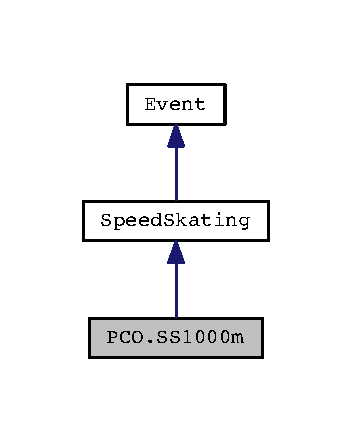
\includegraphics[width=169pt]{classPCO_1_1SS1000m__inherit__graph}
\end{center}
\end{figure}


Collaboration diagram for P\+C\+O.\+S\+S1000m\+:\nopagebreak
\begin{figure}[H]
\begin{center}
\leavevmode
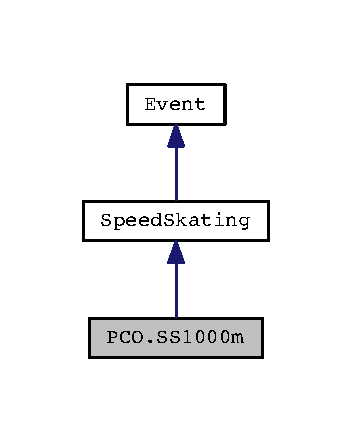
\includegraphics[width=169pt]{classPCO_1_1SS1000m__coll__graph}
\end{center}
\end{figure}
\subsection*{Public Member Functions}
\begin{DoxyCompactItemize}
\item 
\hyperlink{classPCO_1_1SS1000m_a4e960f497e8a5e1f685966fe258974a3}{S\+S1000m} ()
\item 
override double \hyperlink{classPCO_1_1SS1000m_a20cf8a97d91bb661439b1c251942b68a}{ss\+Time} ()
\item 
override int \hyperlink{classPCO_1_1SS1000m_a7087df2094b075191b778e7b56ea07fd}{event\+Num} ()
\item 
override void \hyperlink{classPCO_1_1SS1000m_a00263d1777d343e9485a0da0e5e7f910}{run\+Event} (List$<$ \hyperlink{classPCO_1_1Judge}{Judge} $>$ j, List$<$ \hyperlink{classPCO_1_1Team}{Team} $>$ t)
\item 
override void \hyperlink{classPCO_1_1SS1000m_a883e286f1896171885422cf5c143c2da}{sched\+Event} (List$<$ \hyperlink{classPCO_1_1Judge}{Judge} $>$ j, List$<$ \hyperlink{classPCO_1_1Team}{Team} $>$ t)
\end{DoxyCompactItemize}


\subsection{Detailed Description}
\hyperlink{classPCO_1_1SS1000m}{S\+S1000m} is one of the 3 \hyperlink{classPCO_1_1SpeedSkating}{Speed\+Skating} events. 

D\+E\+F\+I\+N\+T\+I\+O\+N\+: Form of speed skating where athletes utilize inline skates and race around a 400m rink 2.\+5 times. Whichever athlete crosses the finish line first has the lowest time.

C\+O\+N\+S\+T\+R\+A\+I\+N\+T\+S\+: A maximum of four athletes compete at a given time.\begin{DoxyAuthor}{Author}
Landen Marchand 
\end{DoxyAuthor}


Definition at line 15 of file S\+S1000m.\+cs.



\subsection{Constructor \& Destructor Documentation}
\hypertarget{classPCO_1_1SS1000m_a4e960f497e8a5e1f685966fe258974a3}{\index{P\+C\+O\+::\+S\+S1000m@{P\+C\+O\+::\+S\+S1000m}!S\+S1000m@{S\+S1000m}}
\index{S\+S1000m@{S\+S1000m}!P\+C\+O\+::\+S\+S1000m@{P\+C\+O\+::\+S\+S1000m}}
\subsubsection[{S\+S1000m}]{\setlength{\rightskip}{0pt plus 5cm}P\+C\+O.\+S\+S1000m.\+S\+S1000m (
\begin{DoxyParamCaption}
{}
\end{DoxyParamCaption}
)\hspace{0.3cm}{\ttfamily [inline]}}}\label{classPCO_1_1SS1000m_a4e960f497e8a5e1f685966fe258974a3}
Default Constructor Provided Automatically 
\begin{DoxyParams}{Parameters}
{\em None} & \\
\hline
\end{DoxyParams}
\begin{DoxyReturn}{Returns}
Default Values 
\end{DoxyReturn}


Definition at line 21 of file S\+S1000m.\+cs.



\subsection{Member Function Documentation}
\hypertarget{classPCO_1_1SS1000m_a7087df2094b075191b778e7b56ea07fd}{\index{P\+C\+O\+::\+S\+S1000m@{P\+C\+O\+::\+S\+S1000m}!event\+Num@{event\+Num}}
\index{event\+Num@{event\+Num}!P\+C\+O\+::\+S\+S1000m@{P\+C\+O\+::\+S\+S1000m}}
\subsubsection[{event\+Num}]{\setlength{\rightskip}{0pt plus 5cm}override int P\+C\+O.\+S\+S1000m.\+event\+Num (
\begin{DoxyParamCaption}
{}
\end{DoxyParamCaption}
)\hspace{0.3cm}{\ttfamily [inline]}, {\ttfamily [virtual]}}}\label{classPCO_1_1SS1000m_a7087df2094b075191b778e7b56ea07fd}
Function to override inherited \hyperlink{classPCO_1_1SS1000m_a7087df2094b075191b778e7b56ea07fd}{event\+Num()} function 

Implements \hyperlink{classPCO_1_1Event_a89e26f29f5cfc92627bbb5a5e4ca1053}{P\+C\+O.\+Event}.



Definition at line 32 of file S\+S1000m.\+cs.

\hypertarget{classPCO_1_1SS1000m_a00263d1777d343e9485a0da0e5e7f910}{\index{P\+C\+O\+::\+S\+S1000m@{P\+C\+O\+::\+S\+S1000m}!run\+Event@{run\+Event}}
\index{run\+Event@{run\+Event}!P\+C\+O\+::\+S\+S1000m@{P\+C\+O\+::\+S\+S1000m}}
\subsubsection[{run\+Event}]{\setlength{\rightskip}{0pt plus 5cm}override void P\+C\+O.\+S\+S1000m.\+run\+Event (
\begin{DoxyParamCaption}
\item[{List$<$ {\bf Judge} $>$}]{j, }
\item[{List$<$ {\bf Team} $>$}]{t}
\end{DoxyParamCaption}
)\hspace{0.3cm}{\ttfamily [inline]}, {\ttfamily [virtual]}}}\label{classPCO_1_1SS1000m_a00263d1777d343e9485a0da0e5e7f910}
Function to override inherited run\+Event(..) function 

Implements \hyperlink{classPCO_1_1Event_ad47d86904767dfebc731be328ec0958d}{P\+C\+O.\+Event}.



Definition at line 38 of file S\+S1000m.\+cs.

\hypertarget{classPCO_1_1SS1000m_a883e286f1896171885422cf5c143c2da}{\index{P\+C\+O\+::\+S\+S1000m@{P\+C\+O\+::\+S\+S1000m}!sched\+Event@{sched\+Event}}
\index{sched\+Event@{sched\+Event}!P\+C\+O\+::\+S\+S1000m@{P\+C\+O\+::\+S\+S1000m}}
\subsubsection[{sched\+Event}]{\setlength{\rightskip}{0pt plus 5cm}override void P\+C\+O.\+S\+S1000m.\+sched\+Event (
\begin{DoxyParamCaption}
\item[{List$<$ {\bf Judge} $>$}]{j, }
\item[{List$<$ {\bf Team} $>$}]{t}
\end{DoxyParamCaption}
)\hspace{0.3cm}{\ttfamily [inline]}, {\ttfamily [virtual]}}}\label{classPCO_1_1SS1000m_a883e286f1896171885422cf5c143c2da}
Function to override inherited sched\+Event(..) function 

Implements \hyperlink{classPCO_1_1Event_a6a19f71e79d0f498ba74c9cd86c27eaa}{P\+C\+O.\+Event}.



Definition at line 44 of file S\+S1000m.\+cs.

\hypertarget{classPCO_1_1SS1000m_a20cf8a97d91bb661439b1c251942b68a}{\index{P\+C\+O\+::\+S\+S1000m@{P\+C\+O\+::\+S\+S1000m}!ss\+Time@{ss\+Time}}
\index{ss\+Time@{ss\+Time}!P\+C\+O\+::\+S\+S1000m@{P\+C\+O\+::\+S\+S1000m}}
\subsubsection[{ss\+Time}]{\setlength{\rightskip}{0pt plus 5cm}override double P\+C\+O.\+S\+S1000m.\+ss\+Time (
\begin{DoxyParamCaption}
{}
\end{DoxyParamCaption}
)\hspace{0.3cm}{\ttfamily [inline]}, {\ttfamily [virtual]}}}\label{classPCO_1_1SS1000m_a20cf8a97d91bb661439b1c251942b68a}
Function to override inherited \hyperlink{classPCO_1_1SS1000m_a20cf8a97d91bb661439b1c251942b68a}{ss\+Time()} function 

Implements \hyperlink{classPCO_1_1SpeedSkating_a3bc4e4731f04b9ef3d260197ad847117}{P\+C\+O.\+Speed\+Skating}.



Definition at line 26 of file S\+S1000m.\+cs.



The documentation for this class was generated from the following file\+:\begin{DoxyCompactItemize}
\item 
\hyperlink{SS1000m_8cs}{S\+S1000m.\+cs}\end{DoxyCompactItemize}

\hypertarget{classPCO_1_1SS1500m}{\section{P\+C\+O.\+S\+S1500m Class Reference}
\label{classPCO_1_1SS1500m}\index{P\+C\+O.\+S\+S1500m@{P\+C\+O.\+S\+S1500m}}
}


\hyperlink{classPCO_1_1SS1500m}{S\+S1500m} is one of the 3 \hyperlink{classPCO_1_1SpeedSkating}{Speed\+Skating} events.  


\subsection*{Public Member Functions}
\begin{DoxyCompactItemize}
\item 
\hyperlink{classPCO_1_1SS1500m_abcd0ba6477a4d91d5d39031b0fb60d9e}{S\+S1500m} ()
\end{DoxyCompactItemize}


\subsection{Detailed Description}
\hyperlink{classPCO_1_1SS1500m}{S\+S1500m} is one of the 3 \hyperlink{classPCO_1_1SpeedSkating}{Speed\+Skating} events. 

D\+E\+F\+I\+N\+T\+I\+O\+N\+: Form of speed skating where athletes utilize inline skates and race around a 400m rink 3.\+75 times. Whichever athlete crosses the finish line first has the lowest time.

C\+O\+N\+S\+T\+R\+A\+I\+N\+S\+: A maximum of four athletes compete at a given time.\begin{DoxyAuthor}{Author}
Landen Marchand 
\end{DoxyAuthor}


\subsection{Constructor \& Destructor Documentation}
\hypertarget{classPCO_1_1SS1500m_abcd0ba6477a4d91d5d39031b0fb60d9e}{\index{P\+C\+O\+::\+S\+S1500m@{P\+C\+O\+::\+S\+S1500m}!S\+S1500m@{S\+S1500m}}
\index{S\+S1500m@{S\+S1500m}!P\+C\+O\+::\+S\+S1500m@{P\+C\+O\+::\+S\+S1500m}}
\subsubsection[{S\+S1500m}]{\setlength{\rightskip}{0pt plus 5cm}P\+C\+O.\+S\+S1500m.\+S\+S1500m (
\begin{DoxyParamCaption}
{}
\end{DoxyParamCaption}
)\hspace{0.3cm}{\ttfamily [inline]}}}\label{classPCO_1_1SS1500m_abcd0ba6477a4d91d5d39031b0fb60d9e}


The documentation for this class was generated from the following file\+:\begin{DoxyCompactItemize}
\item 
\hyperlink{SS1500m_8cs}{S\+S1500m.\+cs}\end{DoxyCompactItemize}

\hypertarget{classPCO_1_1SS500m}{\section{P\+C\+O.\+S\+S500m Class Reference}
\label{classPCO_1_1SS500m}\index{P\+C\+O.\+S\+S500m@{P\+C\+O.\+S\+S500m}}
}


\hyperlink{classPCO_1_1SS500m}{S\+S500m} is one of the 3 \hyperlink{classPCO_1_1SpeedSkating}{Speed\+Skating} events.  




Inheritance diagram for P\+C\+O.\+S\+S500m\+:\nopagebreak
\begin{figure}[H]
\begin{center}
\leavevmode
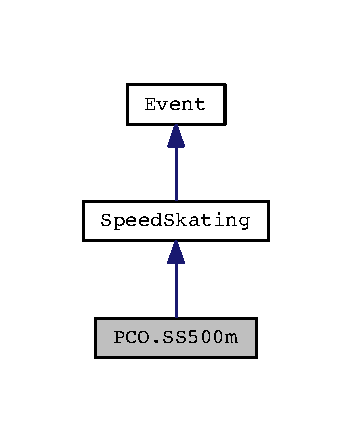
\includegraphics[width=169pt]{classPCO_1_1SS500m__inherit__graph}
\end{center}
\end{figure}


Collaboration diagram for P\+C\+O.\+S\+S500m\+:\nopagebreak
\begin{figure}[H]
\begin{center}
\leavevmode
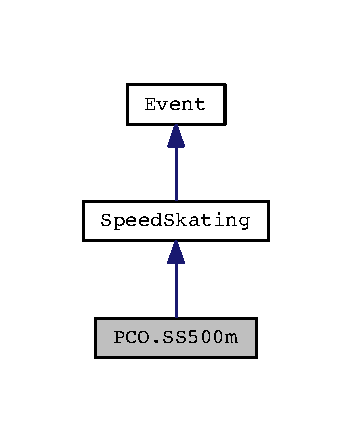
\includegraphics[width=169pt]{classPCO_1_1SS500m__coll__graph}
\end{center}
\end{figure}
\subsection*{Public Member Functions}
\begin{DoxyCompactItemize}
\item 
\hyperlink{classPCO_1_1SS500m_a052125293177cecfa650435ac5decb38}{S\+S500m} ()
\item 
override double \hyperlink{classPCO_1_1SS500m_a57b859e56912c44aee51ac2854f5ce9c}{ss\+Time} ()
\item 
override int \hyperlink{classPCO_1_1SS500m_a909b7bee200b907aae35d8bc47d442e5}{event\+Num} ()
\item 
override void \hyperlink{classPCO_1_1SS500m_a3ebc360a0ec5c60e1d2c66511c8f8025}{run\+Event} (List$<$ \hyperlink{classPCO_1_1Judge}{Judge} $>$ j, List$<$ \hyperlink{classPCO_1_1Team}{Team} $>$ t)
\item 
override void \hyperlink{classPCO_1_1SS500m_a760bbe2b60121e4fe86c64f2c8b60848}{sched\+Event} (List$<$ \hyperlink{classPCO_1_1Judge}{Judge} $>$ j, List$<$ \hyperlink{classPCO_1_1Team}{Team} $>$ t)
\end{DoxyCompactItemize}


\subsection{Detailed Description}
\hyperlink{classPCO_1_1SS500m}{S\+S500m} is one of the 3 \hyperlink{classPCO_1_1SpeedSkating}{Speed\+Skating} events. 

D\+E\+F\+I\+N\+I\+T\+I\+O\+N\+: Form of speed skating where athletes utilize inline skates and race around a 400m rink 1.\+25 times. Whichever athlete crosses the finish line first has the lowest time.

C\+O\+N\+S\+T\+R\+A\+I\+N\+T\+S\+: A maximum of four athletes compete at a given time.\begin{DoxyAuthor}{Author}
Josh King 
\end{DoxyAuthor}


Definition at line 15 of file S\+S500m.\+cs.



\subsection{Constructor \& Destructor Documentation}
\hypertarget{classPCO_1_1SS500m_a052125293177cecfa650435ac5decb38}{\index{P\+C\+O\+::\+S\+S500m@{P\+C\+O\+::\+S\+S500m}!S\+S500m@{S\+S500m}}
\index{S\+S500m@{S\+S500m}!P\+C\+O\+::\+S\+S500m@{P\+C\+O\+::\+S\+S500m}}
\subsubsection[{S\+S500m}]{\setlength{\rightskip}{0pt plus 5cm}P\+C\+O.\+S\+S500m.\+S\+S500m (
\begin{DoxyParamCaption}
{}
\end{DoxyParamCaption}
)\hspace{0.3cm}{\ttfamily [inline]}}}\label{classPCO_1_1SS500m_a052125293177cecfa650435ac5decb38}
Default Constructor Provided Automatically 
\begin{DoxyParams}{Parameters}
{\em None} & \\
\hline
\end{DoxyParams}
\begin{DoxyReturn}{Returns}
Default Values 
\end{DoxyReturn}


Definition at line 21 of file S\+S500m.\+cs.



\subsection{Member Function Documentation}
\hypertarget{classPCO_1_1SS500m_a909b7bee200b907aae35d8bc47d442e5}{\index{P\+C\+O\+::\+S\+S500m@{P\+C\+O\+::\+S\+S500m}!event\+Num@{event\+Num}}
\index{event\+Num@{event\+Num}!P\+C\+O\+::\+S\+S500m@{P\+C\+O\+::\+S\+S500m}}
\subsubsection[{event\+Num}]{\setlength{\rightskip}{0pt plus 5cm}override int P\+C\+O.\+S\+S500m.\+event\+Num (
\begin{DoxyParamCaption}
{}
\end{DoxyParamCaption}
)\hspace{0.3cm}{\ttfamily [inline]}, {\ttfamily [virtual]}}}\label{classPCO_1_1SS500m_a909b7bee200b907aae35d8bc47d442e5}
Function to override inherited \hyperlink{classPCO_1_1SS500m_a909b7bee200b907aae35d8bc47d442e5}{event\+Num()} function 

Implements \hyperlink{classPCO_1_1Event_a89e26f29f5cfc92627bbb5a5e4ca1053}{P\+C\+O.\+Event}.



Definition at line 32 of file S\+S500m.\+cs.

\hypertarget{classPCO_1_1SS500m_a3ebc360a0ec5c60e1d2c66511c8f8025}{\index{P\+C\+O\+::\+S\+S500m@{P\+C\+O\+::\+S\+S500m}!run\+Event@{run\+Event}}
\index{run\+Event@{run\+Event}!P\+C\+O\+::\+S\+S500m@{P\+C\+O\+::\+S\+S500m}}
\subsubsection[{run\+Event}]{\setlength{\rightskip}{0pt plus 5cm}override void P\+C\+O.\+S\+S500m.\+run\+Event (
\begin{DoxyParamCaption}
\item[{List$<$ {\bf Judge} $>$}]{j, }
\item[{List$<$ {\bf Team} $>$}]{t}
\end{DoxyParamCaption}
)\hspace{0.3cm}{\ttfamily [inline]}, {\ttfamily [virtual]}}}\label{classPCO_1_1SS500m_a3ebc360a0ec5c60e1d2c66511c8f8025}
Function to override inherited run\+Event(..) function 

Implements \hyperlink{classPCO_1_1Event_ad47d86904767dfebc731be328ec0958d}{P\+C\+O.\+Event}.



Definition at line 38 of file S\+S500m.\+cs.

\hypertarget{classPCO_1_1SS500m_a760bbe2b60121e4fe86c64f2c8b60848}{\index{P\+C\+O\+::\+S\+S500m@{P\+C\+O\+::\+S\+S500m}!sched\+Event@{sched\+Event}}
\index{sched\+Event@{sched\+Event}!P\+C\+O\+::\+S\+S500m@{P\+C\+O\+::\+S\+S500m}}
\subsubsection[{sched\+Event}]{\setlength{\rightskip}{0pt plus 5cm}override void P\+C\+O.\+S\+S500m.\+sched\+Event (
\begin{DoxyParamCaption}
\item[{List$<$ {\bf Judge} $>$}]{j, }
\item[{List$<$ {\bf Team} $>$}]{t}
\end{DoxyParamCaption}
)\hspace{0.3cm}{\ttfamily [inline]}, {\ttfamily [virtual]}}}\label{classPCO_1_1SS500m_a760bbe2b60121e4fe86c64f2c8b60848}
Function to override inherited sched\+Event(..) function 

Implements \hyperlink{classPCO_1_1Event_a6a19f71e79d0f498ba74c9cd86c27eaa}{P\+C\+O.\+Event}.



Definition at line 44 of file S\+S500m.\+cs.

\hypertarget{classPCO_1_1SS500m_a57b859e56912c44aee51ac2854f5ce9c}{\index{P\+C\+O\+::\+S\+S500m@{P\+C\+O\+::\+S\+S500m}!ss\+Time@{ss\+Time}}
\index{ss\+Time@{ss\+Time}!P\+C\+O\+::\+S\+S500m@{P\+C\+O\+::\+S\+S500m}}
\subsubsection[{ss\+Time}]{\setlength{\rightskip}{0pt plus 5cm}override double P\+C\+O.\+S\+S500m.\+ss\+Time (
\begin{DoxyParamCaption}
{}
\end{DoxyParamCaption}
)\hspace{0.3cm}{\ttfamily [inline]}, {\ttfamily [virtual]}}}\label{classPCO_1_1SS500m_a57b859e56912c44aee51ac2854f5ce9c}
Function to override inherited \hyperlink{classPCO_1_1SS500m_a57b859e56912c44aee51ac2854f5ce9c}{ss\+Time()} function 

Implements \hyperlink{classPCO_1_1SpeedSkating_a3bc4e4731f04b9ef3d260197ad847117}{P\+C\+O.\+Speed\+Skating}.



Definition at line 26 of file S\+S500m.\+cs.



The documentation for this class was generated from the following file\+:\begin{DoxyCompactItemize}
\item 
\hyperlink{SS500m_8cs}{S\+S500m.\+cs}\end{DoxyCompactItemize}

\hypertarget{classPCO_1_1Team}{\section{P\+C\+O.\+Team Class Reference}
\label{classPCO_1_1Team}\index{P\+C\+O.\+Team@{P\+C\+O.\+Team}}
}


\hyperlink{classPCO_1_1Team}{Team} class to house the team name.  


\subsection*{Public Member Functions}
\begin{DoxyCompactItemize}
\item 
\hyperlink{classPCO_1_1Team_a90aa98cc87012423a1ea29958ec92cbf}{Team} ()
\end{DoxyCompactItemize}


\subsection{Detailed Description}
\hyperlink{classPCO_1_1Team}{Team} class to house the team name. 

D\+E\+F\+I\+N\+I\+T\+I\+O\+N\+: Represents each country in the Winter Olympics.

C\+O\+N\+S\+T\+R\+A\+I\+N\+T\+S\+: There must be the same amount of males as females in a team. There is to only be one country per team.\begin{DoxyAuthor}{Author}
Landen Marchand 
\end{DoxyAuthor}


\subsection{Constructor \& Destructor Documentation}
\hypertarget{classPCO_1_1Team_a90aa98cc87012423a1ea29958ec92cbf}{\index{P\+C\+O\+::\+Team@{P\+C\+O\+::\+Team}!Team@{Team}}
\index{Team@{Team}!P\+C\+O\+::\+Team@{P\+C\+O\+::\+Team}}
\subsubsection[{Team}]{\setlength{\rightskip}{0pt plus 5cm}P\+C\+O.\+Team.\+Team (
\begin{DoxyParamCaption}
{}
\end{DoxyParamCaption}
)\hspace{0.3cm}{\ttfamily [inline]}}}\label{classPCO_1_1Team_a90aa98cc87012423a1ea29958ec92cbf}


The documentation for this class was generated from the following file\+:\begin{DoxyCompactItemize}
\item 
\hyperlink{Team_8cs}{Team.\+cs}\end{DoxyCompactItemize}

\chapter{File Documentation}
\hypertarget{Athlete_8cs}{\section{Athlete.\+cs File Reference}
\label{Athlete_8cs}\index{Athlete.\+cs@{Athlete.\+cs}}
}
\subsection*{Classes}
\begin{DoxyCompactItemize}
\item 
class \hyperlink{classPCO_1_1Athlete}{P\+C\+O.\+Athlete}
\begin{DoxyCompactList}\small\item\em \hyperlink{classPCO_1_1Athlete}{Athlete} class to input individual's personal information and events to partake in. \end{DoxyCompactList}\end{DoxyCompactItemize}
\subsection*{Namespaces}
\begin{DoxyCompactItemize}
\item 
package \hyperlink{namespacePCO}{P\+C\+O}
\end{DoxyCompactItemize}

\hypertarget{Database_8cs}{\section{Database.\+cs File Reference}
\label{Database_8cs}\index{Database.\+cs@{Database.\+cs}}
}
\subsection*{Classes}
\begin{DoxyCompactItemize}
\item 
class \hyperlink{classPCO_1_1Database}{P\+C\+O.\+Database}
\begin{DoxyCompactList}\small\item\em D\+E\+P\+R\+E\+C\+A\+T\+E\+D!!! \hyperlink{classPCO_1_1Database}{Database} S\+U\+B\+S\+Y\+S\+T\+E\+M houses all the information of the Winter Olympics. \end{DoxyCompactList}\end{DoxyCompactItemize}
\subsection*{Namespaces}
\begin{DoxyCompactItemize}
\item 
package \hyperlink{namespacePCO}{P\+C\+O}
\end{DoxyCompactItemize}

\hypertarget{Event_8cs}{}\section{Event.\+cs File Reference}
\label{Event_8cs}\index{Event.\+cs@{Event.\+cs}}
\subsection*{Classes}
\begin{DoxyCompactItemize}
\item 
class \hyperlink{classPCO_1_1__0_1_1RegisterEventForm}{P\+C\+O.\+\_\+0.\+Register\+Event\+Form}
\begin{DoxyCompactList}\small\item\em Register Event class for G\+UI. \end{DoxyCompactList}\end{DoxyCompactItemize}
\subsection*{Namespaces}
\begin{DoxyCompactItemize}
\item 
namespace \hyperlink{namespacePCO_1_1__0}{P\+C\+O.\+\_\+0}
\end{DoxyCompactItemize}

\hypertarget{FigureSkating_8cs}{\section{Figure\+Skating.\+cs File Reference}
\label{FigureSkating_8cs}\index{Figure\+Skating.\+cs@{Figure\+Skating.\+cs}}
}
\subsection*{Classes}
\begin{DoxyCompactItemize}
\item 
class \hyperlink{classPCO_1_1FigureSkating}{P\+C\+O.\+Figure\+Skating}
\begin{DoxyCompactList}\small\item\em \hyperlink{classPCO_1_1FigureSkating}{Figure\+Skating} class is the superclass of the 3 \hyperlink{classPCO_1_1FigureSkating}{Figure\+Skating} events. \end{DoxyCompactList}\item 
interface \hyperlink{interfacePCO_1_1FigureSkating_1_1fsInheritance}{P\+C\+O.\+Figure\+Skating.\+fs\+Inheritance}
\end{DoxyCompactItemize}
\subsection*{Namespaces}
\begin{DoxyCompactItemize}
\item 
package \hyperlink{namespacePCO}{P\+C\+O}
\end{DoxyCompactItemize}

\hypertarget{IceDance_8cs}{\section{Ice\+Dance.\+cs File Reference}
\label{IceDance_8cs}\index{Ice\+Dance.\+cs@{Ice\+Dance.\+cs}}
}
\subsection*{Classes}
\begin{DoxyCompactItemize}
\item 
class \hyperlink{classPCO_1_1IceDance}{P\+C\+O.\+Ice\+Dance}
\begin{DoxyCompactList}\small\item\em \hyperlink{classPCO_1_1IceDance}{Ice\+Dance} class is one of the 3 \hyperlink{classPCO_1_1FigureSkating}{Figure\+Skating} events. \end{DoxyCompactList}\end{DoxyCompactItemize}
\subsection*{Namespaces}
\begin{DoxyCompactItemize}
\item 
package \hyperlink{namespacePCO}{P\+C\+O}
\end{DoxyCompactItemize}

\hypertarget{Judge_8cs}{}\section{Judge.\+cs File Reference}
\label{Judge_8cs}\index{Judge.\+cs@{Judge.\+cs}}
\subsection*{Classes}
\begin{DoxyCompactItemize}
\item 
class \hyperlink{classPCO_1_1ScoringForm}{P\+C\+O.\+Scoring\+Form}
\begin{DoxyCompactList}\small\item\em \hyperlink{classScoring}{Scoring} class for G\+UI. \end{DoxyCompactList}\end{DoxyCompactItemize}
\subsection*{Namespaces}
\begin{DoxyCompactItemize}
\item 
namespace \hyperlink{namespacePCO}{P\+CO}
\end{DoxyCompactItemize}

\hypertarget{PairSkating_8cs}{\section{Pair\+Skating.\+cs File Reference}
\label{PairSkating_8cs}\index{Pair\+Skating.\+cs@{Pair\+Skating.\+cs}}
}
\subsection*{Classes}
\begin{DoxyCompactItemize}
\item 
class \hyperlink{classPCO_1_1PairSkating}{P\+C\+O.\+Pair\+Skating}
\begin{DoxyCompactList}\small\item\em \hyperlink{classPCO_1_1PairSkating}{Pair\+Skating} class is one of the 3 \hyperlink{classPCO_1_1FigureSkating}{Figure\+Skating} events. \end{DoxyCompactList}\end{DoxyCompactItemize}
\subsection*{Namespaces}
\begin{DoxyCompactItemize}
\item 
package \hyperlink{namespacePCO}{P\+C\+O}
\end{DoxyCompactItemize}

\hypertarget{Program_8cs}{}\section{Program.\+cs File Reference}
\label{Program_8cs}\index{Program.\+cs@{Program.\+cs}}
\subsection*{Classes}
\begin{DoxyCompactItemize}
\item 
class {\bfseries P\+C\+O.\+Program}
\end{DoxyCompactItemize}
\subsection*{Namespaces}
\begin{DoxyCompactItemize}
\item 
namespace \hyperlink{namespacePCO}{P\+CO}
\end{DoxyCompactItemize}

\hypertarget{Registration_8cs}{}\section{Registration.\+cs File Reference}
\label{Registration_8cs}\index{Registration.\+cs@{Registration.\+cs}}
\subsection*{Classes}
\begin{DoxyCompactItemize}
\item 
class \hyperlink{classPCO_1_1__0_1_1AthleteForm}{P\+C\+O.\+\_\+0.\+Athlete\+Form}
\begin{DoxyCompactList}\small\item\em \hyperlink{classRegistration}{Registration} class for G\+UI. \end{DoxyCompactList}\end{DoxyCompactItemize}
\subsection*{Namespaces}
\begin{DoxyCompactItemize}
\item 
namespace \hyperlink{namespacePCO_1_1__0}{P\+C\+O.\+\_\+0}
\end{DoxyCompactItemize}

\hypertarget{Rink_8cs}{\section{Rink.\+cs File Reference}
\label{Rink_8cs}\index{Rink.\+cs@{Rink.\+cs}}
}
\subsection*{Classes}
\begin{DoxyCompactItemize}
\item 
class \hyperlink{classPCO_1_1Rink}{P\+C\+O.\+Rink}
\begin{DoxyCompactList}\small\item\em \hyperlink{classPCO_1_1Rink}{Rink} class is the physical area in which events are held. \end{DoxyCompactList}\end{DoxyCompactItemize}
\subsection*{Namespaces}
\begin{DoxyCompactItemize}
\item 
package \hyperlink{namespacePCO}{P\+C\+O}
\end{DoxyCompactItemize}

\hypertarget{Schedule_8cs}{\section{Schedule.\+cs File Reference}
\label{Schedule_8cs}\index{Schedule.\+cs@{Schedule.\+cs}}
}
\subsection*{Classes}
\begin{DoxyCompactItemize}
\item 
class \hyperlink{classPCO_1_1Schedule}{P\+C\+O.\+Schedule}
\begin{DoxyCompactList}\small\item\em \hyperlink{classPCO_1_1Schedule}{Schedule} class is the organization of athletes and events. \end{DoxyCompactList}\end{DoxyCompactItemize}
\subsection*{Namespaces}
\begin{DoxyCompactItemize}
\item 
package \hyperlink{namespacePCO}{P\+C\+O}
\end{DoxyCompactItemize}

\hypertarget{Scoring_8cs}{\section{Scoring.\+cs File Reference}
\label{Scoring_8cs}\index{Scoring.\+cs@{Scoring.\+cs}}
}
\subsection*{Classes}
\begin{DoxyCompactItemize}
\item 
class \hyperlink{classPCO_1_1Scoring}{P\+C\+O.\+Scoring}
\begin{DoxyCompactList}\small\item\em \hyperlink{classPCO_1_1Scoring}{Scoring} class manages the official scores/times recorded by the judges. \end{DoxyCompactList}\end{DoxyCompactItemize}
\subsection*{Namespaces}
\begin{DoxyCompactItemize}
\item 
package \hyperlink{namespacePCO}{P\+C\+O}
\end{DoxyCompactItemize}

\hypertarget{SingleSkating_8cs}{\section{Single\+Skating.\+cs File Reference}
\label{SingleSkating_8cs}\index{Single\+Skating.\+cs@{Single\+Skating.\+cs}}
}
\subsection*{Classes}
\begin{DoxyCompactItemize}
\item 
class \hyperlink{classPCO_1_1SingleSkating}{P\+C\+O.\+Single\+Skating}
\begin{DoxyCompactList}\small\item\em \hyperlink{classPCO_1_1SingleSkating}{Single\+Skating} class is one of the 3 \hyperlink{classPCO_1_1FigureSkating}{Figure\+Skating} events. \end{DoxyCompactList}\end{DoxyCompactItemize}
\subsection*{Namespaces}
\begin{DoxyCompactItemize}
\item 
package \hyperlink{namespacePCO}{P\+C\+O}
\end{DoxyCompactItemize}

\hypertarget{SpeedSkating_8cs}{\section{Speed\+Skating.\+cs File Reference}
\label{SpeedSkating_8cs}\index{Speed\+Skating.\+cs@{Speed\+Skating.\+cs}}
}
\subsection*{Classes}
\begin{DoxyCompactItemize}
\item 
class \hyperlink{classPCO_1_1SpeedSkating}{P\+C\+O.\+Speed\+Skating}
\begin{DoxyCompactList}\small\item\em \hyperlink{classPCO_1_1SpeedSkating}{Speed\+Skating} class is the superclass of the 3 \hyperlink{classPCO_1_1SpeedSkating}{Speed\+Skating} events. \end{DoxyCompactList}\end{DoxyCompactItemize}
\subsection*{Namespaces}
\begin{DoxyCompactItemize}
\item 
package \hyperlink{namespacePCO}{P\+C\+O}
\end{DoxyCompactItemize}

\hypertarget{SS1000m_8cs}{\section{S\+S1000m.\+cs File Reference}
\label{SS1000m_8cs}\index{S\+S1000m.\+cs@{S\+S1000m.\+cs}}
}
\subsection*{Classes}
\begin{DoxyCompactItemize}
\item 
class \hyperlink{classPCO_1_1SS1000m}{P\+C\+O.\+S\+S1000m}
\begin{DoxyCompactList}\small\item\em \hyperlink{classPCO_1_1SS1000m}{S\+S1000m} is one of the 3 \hyperlink{classPCO_1_1SpeedSkating}{Speed\+Skating} events. \end{DoxyCompactList}\end{DoxyCompactItemize}
\subsection*{Namespaces}
\begin{DoxyCompactItemize}
\item 
package \hyperlink{namespacePCO}{P\+C\+O}
\end{DoxyCompactItemize}

\hypertarget{SS1500m_8cs}{\section{S\+S1500m.\+cs File Reference}
\label{SS1500m_8cs}\index{S\+S1500m.\+cs@{S\+S1500m.\+cs}}
}
\subsection*{Classes}
\begin{DoxyCompactItemize}
\item 
class \hyperlink{classPCO_1_1SS1500m}{P\+C\+O.\+S\+S1500m}
\begin{DoxyCompactList}\small\item\em \hyperlink{classPCO_1_1SS1500m}{S\+S1500m} is one of the 3 \hyperlink{classPCO_1_1SpeedSkating}{Speed\+Skating} events. \end{DoxyCompactList}\end{DoxyCompactItemize}
\subsection*{Namespaces}
\begin{DoxyCompactItemize}
\item 
package \hyperlink{namespacePCO}{P\+C\+O}
\end{DoxyCompactItemize}

\hypertarget{SS500m_8cs}{\section{S\+S500m.\+cs File Reference}
\label{SS500m_8cs}\index{S\+S500m.\+cs@{S\+S500m.\+cs}}
}
\subsection*{Classes}
\begin{DoxyCompactItemize}
\item 
class \hyperlink{classPCO_1_1SS500m}{P\+C\+O.\+S\+S500m}
\begin{DoxyCompactList}\small\item\em \hyperlink{classPCO_1_1SS500m}{S\+S500m} is one of the 3 \hyperlink{classPCO_1_1SpeedSkating}{Speed\+Skating} events. \end{DoxyCompactList}\end{DoxyCompactItemize}
\subsection*{Namespaces}
\begin{DoxyCompactItemize}
\item 
package \hyperlink{namespacePCO}{P\+C\+O}
\end{DoxyCompactItemize}

\hypertarget{Team_8cs}{}\section{Team.\+cs File Reference}
\label{Team_8cs}\index{Team.\+cs@{Team.\+cs}}
\subsection*{Classes}
\begin{DoxyCompactItemize}
\item 
class \hyperlink{classPCO_1_1__0_1_1TeamForm}{P\+C\+O.\+\_\+0.\+Team\+Form}
\begin{DoxyCompactList}\small\item\em \hyperlink{classTeam}{Team} class for G\+UI. \end{DoxyCompactList}\end{DoxyCompactItemize}
\subsection*{Namespaces}
\begin{DoxyCompactItemize}
\item 
namespace \hyperlink{namespacePCO_1_1__0}{P\+C\+O.\+\_\+0}
\end{DoxyCompactItemize}

%--- End generated contents ---

% Index
\newpage
\phantomsection
\addcontentsline{toc}{chapter}{Index}
\printindex

\end{document}
